\documentclass[preprint]{elsarticle}\usepackage[]{graphicx}\usepackage[]{color}
%% maxwidth is the original width if it is less than linewidth
%% otherwise use linewidth (to make sure the graphics do not exceed the margin)
\makeatletter
\def\maxwidth{ %
  \ifdim\Gin@nat@width>\linewidth
    \linewidth
  \else
    \Gin@nat@width
  \fi
}
\makeatother

\definecolor{fgcolor}{rgb}{0.345, 0.345, 0.345}
\newcommand{\hlnum}[1]{\textcolor[rgb]{0.686,0.059,0.569}{#1}}%
\newcommand{\hlstr}[1]{\textcolor[rgb]{0.192,0.494,0.8}{#1}}%
\newcommand{\hlcom}[1]{\textcolor[rgb]{0.678,0.584,0.686}{\textit{#1}}}%
\newcommand{\hlopt}[1]{\textcolor[rgb]{0,0,0}{#1}}%
\newcommand{\hlstd}[1]{\textcolor[rgb]{0.345,0.345,0.345}{#1}}%
\newcommand{\hlkwa}[1]{\textcolor[rgb]{0.161,0.373,0.58}{\textbf{#1}}}%
\newcommand{\hlkwb}[1]{\textcolor[rgb]{0.69,0.353,0.396}{#1}}%
\newcommand{\hlkwc}[1]{\textcolor[rgb]{0.333,0.667,0.333}{#1}}%
\newcommand{\hlkwd}[1]{\textcolor[rgb]{0.737,0.353,0.396}{\textbf{#1}}}%
\let\hlipl\hlkwb

\usepackage{framed}
\makeatletter
\newenvironment{kframe}{%
 \def\at@end@of@kframe{}%
 \ifinner\ifhmode%
  \def\at@end@of@kframe{\end{minipage}}%
  \begin{minipage}{\columnwidth}%
 \fi\fi%
 \def\FrameCommand##1{\hskip\@totalleftmargin \hskip-\fboxsep
 \colorbox{shadecolor}{##1}\hskip-\fboxsep
     % There is no \\@totalrightmargin, so:
     \hskip-\linewidth \hskip-\@totalleftmargin \hskip\columnwidth}%
 \MakeFramed {\advance\hsize-\width
   \@totalleftmargin\z@ \linewidth\hsize
   \@setminipage}}%
 {\par\unskip\endMakeFramed%
 \at@end@of@kframe}
\makeatother

\definecolor{shadecolor}{rgb}{.97, .97, .97}
\definecolor{messagecolor}{rgb}{0, 0, 0}
\definecolor{warningcolor}{rgb}{1, 0, 1}
\definecolor{errorcolor}{rgb}{1, 0, 0}
\newenvironment{knitrout}{}{} % an empty environment to be redefined in TeX

\usepackage{alltt}
\usepackage[paperwidth=8.5in,paperheight=11in,top=1in,bottom=1in,left=1in,right=1in]{geometry}
\usepackage{setspace}
\usepackage[colorlinks=true,allcolors=Blue]{hyperref}
\usepackage{lineno}
\usepackage{cleveref}
\usepackage{acronym}
\usepackage{paralist}
\usepackage{bm}
\usepackage{fixltx2e}
% \usepackage[inline]{showlabels}

\journal{Ecological Modelling}

% biblio options
\bibliographystyle{elsarticle-harv}
\biboptions{authoryear}

% cleveref options
\crefname{table}{Table}{Tables}
\crefname{figure}{Fig.}{Figs.}
\renewcommand{\figurename}{Fig.}

% aliased citations
\defcitealias{LehrterIP}{Lehrter et al. in press}

%acronyms
\acrodef{chla}[chl-\textit{a}]{chlorophyll \textit{a}}
\acrodef{cgem}[CGEM]{Coastal General Ecosystem Model}
\acrodef{do}[O$_2$]{dissolved oxygen}
\acrodef{dom}[DOM]{dissolved organic matter}
\acrodef{gom}[GOM]{Gulf of Mexico}
\acrodef{lcs}[LCS]{Louisiana continental shelf}
\acrodef{marb}[MARB]{Mississippi-Atchafalaya River Basin}
\acrodef{pom}[POM]{particulate organic matter}
\acrodef{zerod}[0-D]{zero-dimensional}

%for supplemental figures/tables
\newcommand{\beginsupplement}{%
        \setcounter{table}{0}
        \renewcommand{\thetable}{S\arabic{table}}%
        \setcounter{figure}{0}
        \renewcommand{\thefigure}{S\arabic{figure}}%
     }

% invisible section anchor
\newcommand\invisiblesection[1]{%
  \refstepcounter{section}%
  \addcontentsline{toc}{section}{\protect\numberline{\thesection}#1}%
  \sectionmark{#1}}

% macro fix for multiple asterisks for corr author
\makeatletter
\def\@author#1{\g@addto@macro\elsauthors{\normalsize%
    \def\baselinestretch{1}%
    \upshape\authorsep#1\unskip\textsuperscript{%
      \ifx\@fnmark\@empty\else\unskip\sep\@fnmark\let\sep=,\fi
      \ifx\@corref\@empty\else\unskip\sep\@corref\let\sep=,\fi
      }%
    \def\authorsep{\unskip,\space}%
    \global\let\@fnmark\@empty
    \global\let\@corref\@empty  %% Added
    \global\let\sep\@empty}%
    \@eadauthor={#1}
}
\makeatother

% fix warning if acronyms are reset after abstract
\makeatletter
\renewcommand*\@verridelabel[1]{%
  \@bsphack
  \protected@write\@auxout{}{\string\undonewlabel{#1}}%
  \protected@write\@auxout{}{\string\undonewlabel{#1@cref}}%Added for cleverref
  \label{#1}%
  \@overriddenmessage rs{#1}%
  \@esphack
}%
\makeatother

\linespread{1.5}

%knitr options


% R dependencies


% get the version from git log


% get online bib file


\IfFileExists{upquote.sty}{\usepackage{upquote}}{}
\begin{document}

\begin{frontmatter}

\title{Parameter sensitivity and identifiability for a biogeochemical model of hypoxia in the northern {G}ulf of {M}exico\tnoteref{mytitlenote}}
\tnotetext[mytitlenote]{Version: Thu Mar 9 13:12:38 2017 -0600, \href{https://github.com/fawda123/identifiability/commit/70c8da3c6d4aa0e50231198ae90027a250ce2ae5}{70c8da3c6d4aa0e50231198ae90027a250ce2ae5}}

\date{}

\author{Marcus W. Beck\corref{mycorrespondingauthor}}
\address{USEPA National Health and Environmental Effects Research Laboratory, Gulf Ecology Division, 1 Sabine Island Drive, Gulf Breeze, FL 32561}
\cortext[mycorrespondingauthor]{Corresponding author}
\ead{beck.marcus@epa.gov}

\author{John C. Lehrter}
\address{Dauphin Island Sea Lab, University of South Alabama, Dauphin Island, AL 36528}
\ead{jlehrter@disl.org}

\author{Lisa L. Lowe}
\address{Lockheed Martin IS \& GS - Civil supporting the USEPA, Research Triangle Park, NC 27709}
\ead{lowe.lisa@epa.gov}

\author{Brandon M. Jarvis}
\address{USEPA National Health and Environmental Effects Research Laboratory, Gulf Ecology Division, 1 Sabine Island Drive, Gulf Breeze, FL 32561}
\ead{jarvis.brandon@epa.gov}

\begin{abstract}
\noindent This study addresses quantitative limitations of coupled hydrodynamic-ecological models by evaluating parameter sensitivity and identifability of a \ac{zerod} unit of a larger spatio-temporal model of hypoxia on the \acl{lcs} of Gulf of Mexico.  A systematic framework is used to infer larger trends in dissolved oxygen dynamics over time, having implications for understanding factors that contribute to environmental conditions that are detrimental to aquatic resources.  In particular, we focus on issues of parameter identifiability using local sensitivity analyses to provide quantitative descriptions of numerical constraints on model precision.  The sensitivity of state variables differed considerably with parameter changes, although most variables were responsive to changes in parameters that influenced planktonic growth rates and less sensitive to physical or chemical parameters.  Variation in sensitivity had a direct correspendence with identifiability, such that only small subsets of the complete parameter set were characterized as having unique effects on the model output. As a result, we provide a set of parameter selection heuristics that can be used to identify parameters for model calibration that depend on relative sensitivity and ecological categories within the biogeochemical equations. Although these concerns have been expressed in the literature, they are rarely explicitly addressed or included in evaluations of water quality models.
\end{abstract}

\begin{keyword}
\ac{cgem}, \ac{gom}, Hypoxia, Identifiability, Sensitivity
\end{keyword}

\end{frontmatter}

\linenumbers
\acresetall

\section{Introduction}

Hypoxia formation in bottom waters of coastal oceans occurs primarily from excess nutrient inputs from land-based sources \citep{Justic87,Diaz95,Howarth96}.  These events are detrimental to aquatic organisms and have significant negative effects on economic resources derived from coastal ecosystems \citep{Lipton03,Diaz11}.  An understanding of the biological, physical, and chemical processes that contribute to the growth of hypoxic areas is a critical concern for mitigating and preventing these negative impacts.  Numerical ecosystem models are important tools that synthesize knowledge of ecosystem processes that contribute to hypoxia formation and for predicting the effects of proposed management activities or future scenarios \citep{Scavia04,Hagy07,Pauer16}.  Unlike statistical models with more generic structures, simulation and process-based models include explicit descriptions of relevant processes that are constrained by empirical or observational data relevant to the system of interest \citep[e.g.][]{Omlin01b,Eldridge10}.  These models are often coupled with hydrodynamic grids to provide spatially-explicit representations of patterns in three dimensions \citep{Warner05,Zhao10,Ganju16}. Combined hydrodynamic and bio-geo-chemical models have been developed specifically to describe hypoxic conditions on the \ac{lcs} in the northern \ac{gom} (\citealt{Fennel13,Obenour15,Pauer16}, \citetalias{LehrterIP}).  This area drains a significant portion of the continental United States through the \ac{marb} and is the second largest hypoxic area in the world \citep{Rabalais02}.  Understanding processes that contribute to the frequency and duration of hypoxic events remains a critical research goal for the region.  

The development and application of a model represents a tradeoff between characteristics expected from the output or provided by the structural components. An idealized model is sufficiently generalizable across systems, provides results that are precise given the inputs, and includes components that are realistic descriptions of actual processes \citep{Levins66}. Given that these characteristics cannot be simultaneously achieved, models are developed in partial dependence of reality and theoretical constructs, completely separate from both, or dependent on one or the other \citep{Morrison99,Ganju16}.  These challenges are analagous to the well-known bias-variance tradeoff in statistical models that balances the competing objectives of over- and under-fitting to an observed dataset. Process-based models are more commonly imbalanced between reality and theory, such that most are over-parameterized in an attempt to completely describe reality \citep{Denman03,Nossent12,Petrucci14}.  Quantitative limitations of over-parameterization are analagous to degrees of freedom in standard statistical models as free parameters cannot be numerically estimated when constrained to an observed dataset \citep{Kirchner06}.  More importantly, over-parameterization can limit use across systems outside of the data domain and impose uncertainty in model predictions as realistic values for every variable may not be known or inaccurately applied from existing studies \citep{Durand02,Refsgaard07,Wade08}.

Model precision can be evaluated relative to the effects of initial conditions or the observed data used for calibration, changes in parameter values, or variation in the structural components (i.e., observational, parameter, or structural uncertainty) \citep{Beck87}.  Evaluating effects of parameter changes is by far the most common and simplest approach.  Although sensitivity analyses should be integrated with model development, parameters are often evaluated post-hoc as a form of `damage control' for further calibration.  This approach is sometimes called inverse modelling where results from sensitivity analyses are used to guide calibration or fit of the developed model to observations (\citealt{Soetaert10}, or confronting models with data, \textit{sensu} \citealt{Hilborn97}).  Parameter sensitivity analysis combined with inverse modelling necessarily involves questions of parameter `identifiability'.  Redundancies in parameter effects lead to unidentifiable models where calibration is empirically impossible (i.e., standard algorithms will not converge) or parameter values may be non-unique leading to the right answer for the wrong reason \citep{Kirchner06}. Unidentifiable parameter sets have effects on model output that can be undone or compensated for by alteration of other parameters.  Identifiability issues are not foreign to hypoxia or eutrophication models  \citep{Omlin01,Estrada10,Mateus15}, although there is a clear need for greater integration of these concepts in practice \citep{Fasham06}.

This study describes a parameter sensitivity and identifiability analysis of a \ac{zerod} unit of a larger spatial-temporal model of hypoxia dynamics on the \ac{lcs}.  The objectives were to provide a statistical approach that demonstrates numerical limitations of parameter sets for model calibration and provide a framework for selecting parameters within the identifability constraints.  The specific goals were to \begin{inparaenum}[1\upshape)]
\item identify the parameters that have the greatest influence on state variables using local sensitivity analysis,
\item quantify the identifiability of subsets of the total parameter space based on sensitivity,
\item and provide a set of heuristics for choosing parameters based on sensitivity, identifiability, and parameter categories.
\end{inparaenum}
In addition to \ac{do}, other state variables that were evaluated included ammonium, \ac{chla}, irradiance, nitrate, \ac{pom}, \ac{dom}, and phosphorus. In general, we provide empirical results to support the assumption that models are generally over-parameterized and only a finite and smaller subset of the complete parameter set can be optimized. Although concerns of identifiability constraints have been shown in the literature, rulesets are not readily available that define how parameters should be selected given tradeoffs betwen precision, sensitivity, and identifiability, especially for biogeochemical models of ecosystem processes.

\section{Methods}

\subsection{Model description}

Hypoxic events, defined  as $<$2 mg L$^{-1}$ of \ac{do} ($<$ 64 mmol m$^{-3}$), occur seasonally in bottom waters in the northern \ac{gom}.  The hypoxic area averages 15,540 km$^2$ annually (1993-2015) with minimum concentrations observed from late spring to early fall.  Seasonal variation is strongly related to carbon and nutrient export from the \ac{marb} \citep{Lohrenz08,Bianchi10}, whereas hydrologic variation, currents, and wind patterns can affect vertical salinity gradients that contribute to the formation of hypoxia \citep{Wiseman97,Paerl98,Obenour15}. The \ac{cgem} was developed to describe hypoxia dynamics on the \ac{lcs} and includes elements from the Navy Coastal Ocean Model \citep{Martin00} for hydrodynamics and a biogeochemical model with multiple plankton groups, water-column metabolism, and sediment diagenesis \citep{Eldridge10}.  The hydrodynamic component of \ac{cgem} provides a spatially-explicit description of hypoxia using an orthogonal grid with an approximate horizontal resolution of 1.9 km$^2$ and twenty equally-spaced vertical sigma layers on the shelf.  The biogeochemical component includes equations for 36 state variables including six phytoplankton groups (with nitrogen and phosophorus quotas for each), two zooplankton groups, nitrate, ammonium, phosphate, dissolved inorganic carbon, oxygen, silica, and multiple variables for dissolved and particulate organic matter from different sources.

The core unit of \ac{cgem} is FishTank, a \ac{zerod} model that implements the biogeochemical equations in \citet{Eldridge10} and does not include any advection, mixing, or sediment diagenesis. Although FishTank was developed for specific application in \ac{cgem}, it can easily be applied to other hydrodynamic grids. Results are based on time-dependent differential equations that describe energy flow between phytoplankton and zooplankton groups given nutrient uptake rates, organic matter inputs and losses, inherent optical properties, and temperature (\citealt{Penta08,Eldridge10}, see appendix in \citetalias{LehrterIP}). A total of 108 equations are estimated at each time step to return values for each of the 36 state variables described by the model.  In addition to the initial conditions, 251 parameter values for each of the equations are also supplied at model execution. Values for each of the parameters were based on estimates from the literature, field or laboratory-based measurements, or expert knowledge in absence of the former.  As such, a sensitivity analysis of parameter values is warranted given that, for example, literature or field-based estimates may not apply under all scenarios or expert knowledge is not completely certain \citep{Refsgaard07}.

% number of parameters evaluated, total and by category


The sensitivity of state variables to perturbations of all relevant parameters for the 108 equations was estimated using a five minute timestep from January 1\textsuperscript{st} to December 31\textsuperscript{st}, 2006. Irrelevant parameters were removed for several reasons; parameters were not relevant for the \ac{zerod} model (i.e., hydrodynamic parameters), were considered physical constants, or had no effect given initial conditions.  Additionally, FishTank includes six phytoplankton and two zooplankton groups to add complexity in community structure and foodweb dynamics. To remove obvious redundancies, the sensitivity analyses were conducted using only one phytoplankton and one zooplankton group.  The final set that was evaluated included 51 parameters that were further grouped into one of six categories based on applicable biogeochemical components of the model: optics ($n = $ 4 parameters), organic matter (12), phytoplankton (22), temperature (2), and zooplankton (11).  A full description of the model parameters is available as an appendix in \citetalias{LehrterIP}.  

\subsection{Local sensitivity analysis}

A local sensitivity analysis was performed by evaluating the change in state variables following perturbation of each parameter from its original value \citep{Soetaert10,RDCT16}. Parameters were individually perturbed by 50\% of the original values and sensitivity $S$ was estimated for each time step $i$ given a change for parameter $j$ as:

\begin{equation} \label{sijeqn}
S_{ij} = \frac{\partial y_i}{\partial \Theta_j}\cdot\frac{w_{\Theta_j}}{w_{y_i}}
\end{equation}

\noindent where the estimate is based on the change in the predicted value for response variable $y$ divided by the change in the parameter $\Theta_j$ multiplied by the quotient of scaling factors $w$ for each.  The scaling factors, $w_{\Theta_j}$ for the parameter $\Theta_j$ and $w_{y_i}$ for response variable $y_i$, were set as the default value of the unperturbed parameter and the predicted value of $y_i$ after perturbation \citep{Soetaert10}.  Scaling makes the estimates unitless to compare model sensitivity to parameters and state variables that differ in relative magnitude.  Sensitivity values for all $j$ parameters were summarized as a single value across the time series from $i = 1$ to $n$ as $L1$:

\begin{equation} \label{l1}
L1 = \sum|S_{ij}|/n
\end{equation}

All parameters for each of the six equation categories (optics, organic matter, phytoplankton, temperature, and zooplankton) that had non-zero $L1$ were retained for identifiability analysis.  

\subsection{Identifiability and selecting parameter subsets}

The collinearity index $\gamma$ provides a measure of potential redundancies in the response of a state variable to changes in parameter values.  The index measures the linear dependence between sensitivity functions (i.e., $S_i$ for $j$ parameters) described above for parameter subsets and was estimated from the minimum eigenvector of the cross-product of a selected sensitivity matrix \citep{Brun01,Omlin01}:

\begin{equation} \label{gameq}
\gamma = \frac{1} {\sqrt{ \min \left(\rm{EV}[\mathit{\hat{S}}^\top \mathit{\hat{S}}]\right)}}
\end{equation}

\noindent where $\gamma$ ranges from one to infinity for perfectly identifiable (orthogonal) or unidentifiable (perfectly collinear) parameter sets.  The sensitivity functions were supplied as a matrix $\hat{S}$ with rows $i$ and columns $j$ (\cref{sijeqn}) that described deviations of predicted \ac{do} following perturbations of each parameter.  Thus, $\gamma$ can be estimated from results for any subset of parameter combinations. Sensitivity matrices were first normalized by dividing by the square root of the summed residuals \citep{Omlin01,Soetaert10}. Estimates of $\gamma$ greater than 10-15 suggest parameter sets are poorly identifiable \citep{Brun01,Omlin01}, meaning parameter values that maximize precision on a calibration dataset are inestimable by conventional optimization algorithms. An intuitive interpretation of $\gamma$ is provided by \citet{Brun01}, such that a change in a state variable caused by a change in one parameter can be offset by the fraction $1 - 1/\gamma$ by the remaining parameters.  That is, $\gamma = 10$ suggests the relative change in \ac{do} for an arbitrary parameter in the selected set can be compensated for by 90\% with changes in the other parameters. 

Parameter selection for model calibration must consider the competing objectives of increased precision with parameter inclusion and reduced identifability as it relates to optimization.  An additional challenge is a large number of combinations of parameter sets, which complicates selection given sensitivity differences and desired ecological categories of each parameter (e.g., practitioners may only be interested in optics parameters).  \cref{fig:combnex} provides a simple graphic of the unique number of combinations that are possible for different subsets of `complete' parameter sets of different sizes (i.e., $n$ choose $k$ combinations, $n!/\left(k!\left(n-k\right)!\right)$).  The number of unique combinations increases with the total parameters in the set and is also maximized for moderate selections (e.g., selecting half the total).  For example, over 10$^{14}$ combinations are possible by selecting 25 parameters from a set of 50.

A set of heuristics was developed that addresses the tradeoff in model complexity and identifiability given the challenges described above \citep[see also][]{Wagener01}.  These rulesets were developed with the assumption that parameters will be selected with preference for those with high sensitivity and identifability based on $\gamma < 15$ as an acceptable threshold for subsets (e.g., 93\% accountability between parameters).  Selection heurestics also recognized that parameter categories (i.e., optics, organic matter, phytoplankton, temperature, zooplankton) may have unequal preferences by model users given questions of interest.  In all selection scenarios, parameters were selected by decreasing sensitivity starting with the most sensitive until identifiability did not exceed $\gamma = 15$ where selections were \begin{inparaenum}[1\upshape)]
\item blocked within parameter category,
\item independent of parameter category,
\item or considering all categories equally.
\end{inparaenum} The selection rules produced seven subsets of parameters that could further be used to optimize model calibration.

\subsection{Model calibration with parameter subsets}

% we want to show that the results have relevance for the larger three-dimensional model and that model output for calibration to different parameters sets will have differing precision given 1) differences in sensitivity to included ina  subsets and 2) differences given proportion of parameters selected from different categories.  

% we use a time series from Weeks Bay NERRS because data are continuous, initial conditions were modified to match weeks bay conditions.  DO time series was filtered to remove tidal advection component and air/sea gas exhange was used.  This is not a perfect example but works for our purposes to demonstrate differeing precision as directly related to identifiability of subsets and paramter types in a subset. Thus we were primarily concerned with showing differences in calibration results between paramters sets and not an absolute description of the time series.    
% note that we are not concerned with the magnitude of the error but the differences in error between parameter subsets and number of runs to convergence.  

\section{Results}

% for inline

 
\subsection{Local sensitivity analysis}

Local sensitivity analyses showed that \ac{do} was sensitive to perturbations in 38 of the 51 (75\% of total) parameters that were evaluated in FishTank (\cref{fig:sensalltile}, \cref{tab:dosens}). Within each parameter category, \ac{do} was sensitive to three parameters for optics (75\% of all optic parameters), eight for organic matter (67\%), 16 for phytoplankton (73\%), one for temperature (50\%), and 10 for zooplankton (91\%). Although \ac{do} had the greatest sensitivity to parameters in the zooplankton category (as percentage of total), the relative effects varied. Among all parameters, average sensitivity was $L1 = $ $9.2\times 10^{-3}$ with values ranging from $L1 = $ $8.34\times 10^{-8}$ for \textit{QminP} (phytoplankton) to $0.05$ for \textit{umax} (phytoplankton). Within categories (excluding temperature with one sensitive parameter), sensitivity ranged from $4.39\times 10^{-5}$ (\textit{astarOMA}) to $7.51\times 10^{-4}$ (\textit{astar490}) for optics, $4.17\times 10^{-4}$ (\textit{KNH4}) to $6.15\times 10^{-3}$ (\textit{KG1}) for organic matter, $8.34\times 10^{-8}$ (\textit{QminP}) to $0.05$ (\textit{umax}) for phytoplankton, and $3.69\times 10^{-5}$ (\textit{ZQp}) to $0.05$ (\textit{ZKa}) for zooplankton (\cref{tab:dosens}).  Average sensitivity values in each category were $L1 = $ $2.81\times 10^{-4}$ for optics, $2.17\times 10^{-3}$ for organic matter, $0.02$ for temperature, $0.01$ for phytoplankton, and $0.01$ for zooplankton.



Local sensitivity analyses for the additional state variables (ammonium, \ac{chla}, irradiance, nitrate, \ac{pom}, \ac{dom}, and phosphorus) had similar results as \ac{do} with some exceptions (\cref{fig:sensalltile,tab:nh4sens,tab:chlsens,tab:irrsens,tab:no3sens,tab:om1sens,tab:om2sens,tab:po4sens}).  All variables were sensitive to the same parameters as \ac{do} (38 of 51 evaluated), although average sensitivity differed between variables.  Average $L1$ ranged from $0.02$ for irradiance (\cref{tab:irrsens}) to $0.71$ for \ac{dom} (\cref{tab:om2sens}).  All average sensitivity values for the state variables were higher than the average for \ac{do} ($L1$ = $9.2\times 10^{-3}$).  For each variable, $L1$ ranged from $2.24\times 10^{-6}$ (\textit{QminP}) to $8.49$ (\textit{mA}) for ammonium (\cref{tab:nh4sens}), $1.38\times 10^{-6}$ (\textit{QminP}) to $13.94$ (\textit{mA}) for \ac{chla} (\cref{tab:chlsens}), $1.92\times 10^{-7}$ (\textit{QminP}) to $0.13$ (\textit{ZKa}) for irradiance (\cref{tab:irrsens}), $6.67\times 10^{-7}$ (\textit{QminP}) to $8.49$ (\textit{umax}) for nitrate (\cref{tab:no3sens}), $6.41\times 10^{-5}$ (\textit{KNH4}) to $7.22$ (\textit{mA}) for \ac{pom} (\cref{tab:om1sens}),  $7.41\times 10^{-5}$ (\textit{KNH4}) to $14.25$ (\textit{mA}) for \ac{dom} (\cref{tab:om2sens}), and $8.21\times 10^{-7}$ (\textit{QminP}) to $1.47$ (\textit{ZKa}) for phosphate (\cref{tab:po4sens}).  For the parameter categories, ammonium was most sensitive to phytoplankton parameters (average $L1$ = $0.8$ across all parameters in the category), \ac{chla} to phytoplankton ($L1$ = $1.14$), irradiance to zooplankton ($L1$ = $0.03$), nitrate to zooplankton ($L1$ = $1.06$), \ac{pom} to temperature ($L1$ = $0.86$), \ac{dom} to temperature ($L1$ = $1.48$), and phosphate to zooplankton ($L1$ = $0.31$).  Finally, average sensitivity between parameter categories independent of the state variables ranged from $8.38\times 10^{-3}$ for optics (average $L1$ across all variables) to $0.62$ for phytoplankton. 

\subsection{Identifiability of parameter subsets and selection rules}



The identifiability analyses suggested that many parameter subsets exceeded the thresholds of $\gamma = 10, 15$.  Parameter identifiability for \ac{do} decreased (increasing $\gamma$) at different rates with increasing size of parameter subsets depending on the parameter category or the number of top parameters that were selected (\cref{fig:identplo}). By category, identifiability was lowest for all combinations of parameter subsets in the phytoplankton ($60$\% of subsets less than $\gamma = 15$, $43$\% less than $\gamma = 10$) and zooplankton categories ($53.1$\% less than $\gamma = 15$, $40$\% less than $\gamma = 10$), whereas all combinations were identifiable for optics ($100$\% less than $\gamma = 15, 10$) and a majority identifiable for organic matter ($91.9$\% less than $\gamma = 15$, $76.5$\% less than $\gamma = 10$). Identifiability for parameters in the temperature category was not evaluated because \ac{do} was sensitive to only one parameter (i.e., $\gamma = 1$). Parameter combinations for choosing from the top, top two, top three, and top four parameters in each category together had decreasing identifability with the increasing size of the selection pool (e.g., top one versus top four parameters, \cref{fig:identplo}).  The percentage of parameter subsets that were below the acceptable thresholds for identifability was $100$\% less than $\gamma = 15, 10$ for the top parameter in each category, $90.6$\% and $80.7$\% for the top two, $80.7$\% and $70.9$\% for the top three, and $55.8$\% and $45.7$\% for the top four.  Results for the remaining state variables had similar patterns in identifiability with increasing size of parameter subsets and selection categories, although differences in identifiabiltiy between state variables was observed (\cref{fig:identploall}).  Most notably, nitrate was consistently the least identifiable variable (highest overall $\gamma$), whereas \ac{do} was most identifiable.

An alternative view of the results in \cref{fig:identplo} can be used to demonstrate the effects of parameter selection criteria and number of parameters in the selection pool on identifiability.  \Cref{fig:percthresh} shows the percentage of identifiable parameter sets for \ac{do} using the same selection criteria in \cref{fig:identplo}, i.e., selection of parameters only within parameter categories and selection of the top sensitive parameters regardless of category.  \Cref{fig:percthresh} is similar to \cref{fig:identplo}, with the added effect of a chosen $\gamma$ threshold on identifability.  Previous studies have provided only general rules for $\gamma$ thresholds \citep{Brun01,Omlin01}, such that exact values for which parameter sets are inestimable likely vary between models and optimization methods.  As such, multiple values are shown in \cref{fig:percthresh}  given that actual thresholds could vary in practice. In general, identifiability decreased with the addition of parameters, although the rate of decrease depended on the selected threshold for $\gamma$. More conservative values for $\gamma$ (e.g., $\gamma = 5$) were more sensitive to the number of parameters in a subset, that is, identifiability decreased more quickly with the addition of parameters at lower $\gamma$ thresholds as compared to higher $\gamma$.  Notable differences in identifiability were also observed by parameter selection criteria (within categories or top parameters only), which further supports results in \cref{fig:identplo,fig:identploall}.    



An evaluation of the effects of individual parameters on $\gamma$ suggested that some parameters had disproportionate effects on identifiability.  Based on $\gamma = 15$, \cref{fig:identplo} suggests that most parameter sets for organic matter were identifiable, regardless of how many parameters were selected (i.e., two through eight).  However, some subsets were not identifiable such that identification of one or more redundant parameters that are inflating $\gamma$ values could provide useful information.  \Cref{fig:exclex} shows an alternative view of identifiability of \ac{do} with exclusion and inclusion of individual parameters in different sets for the organic matter category.  As before, collinearity increases with more parameters in a subset, although the increase varies depending on which parameter was included or excluded from the set.  For example, inclusion of \textit{KNO3} in a parameter set almost always inflated $\gamma$.  All parameter subsets that did not include \textit{KNO3} were well below $\gamma = 15$, suggesting that exclusion of this parameter improves identifiability.  Interestingly, the inclusion of some parameters caused a reduction in $\gamma$, which contradicts the general rule that more parameters caused reduced identifiablity.  For example, parameter sets that included \textit{KGcdom} generally had lower $\gamma$ values relative to those that excluded the parameter.


Results for each of the three selection heuristics (blocked by parameter category, independent of category, all categories equally) applied to each state variable differed in the number of selected parameters and distribution of parameters within each category (\cref{tab:heurist1,tab:heurist2,tab:heurist3}).  In general, a corresponendence was observed between the number of parameters that were selected given the threhold of $\gamma = 15$ and relative identifiability between the state variables.  As noted above, nitrate was the least identifiable variable (\cref{fig:identploall}), whereas other variables (e.g., \ac{do}, irradiance) were more identifiable.  The constraints on identifiability between variables were demonstrated with the selection heuristics.  For example, heuristics for nitrate typically selected only one or two parameters that met the criteria as compared to more identifiable variables that included several parameters. Overall, the first selection heuristic demonstrated that the number of parameters chosen by parameter category differed independently of the state variables (\cref{tab:heurist1}). The number of selected parameters averaged across state variables in decreasing order was 4.25 parameters from the phytoplankton category, 3.5 from organic matter, 2.75 from optics, and 2.38 from zooplankton. The second and third selection heuristics (\cref{tab:heurist2,tab:heurist3}) were similar, although more parameters were generally selected for the third heuristic given equal importance between categories.

\section{Discussion}

\subsection{Implications of sensitivity and identifiability analyses}

Common goals in the application of biogeochemical models of ecosystem processes are to \begin{inparaenum}[1\upshape)]
\item accurately describe the system by matching predictions with observed data \citep{Reckhow90}, and 
\item provide a means of forecasting ecosystem condition with hypothesized management or environmental scenarios \citep{Clark01}. 
\end{inparaenum}
Although these objectives are the focus of most applications, the structural components of process-based models should secondarily provide inference into which ecosystem processes and functions are driving observed changes.  This latter objective represents a more generic scientific purpose of biogeochemical models that extends beyond the applied benefits of describing and predicting change in a particular system.  Modelers often hope to identify universal principles that govern dynamics across systems and the constraint of model parameters to observations provides a means of supporting or refuting hypotheses \citep{Kirchner06}.  Extension of these principles to test the effects of structural changes and observation uncertainty on model predictions provides further information to support validation of model components. This study provided a simple approach to use the effects of parameter perturbations on model state variables to characterize identifiable parameter subsets that vary by parameter selection criteria.  By doing so, we demonstrated that small parameter subsets relative to all sensitive parameters were within the identifiability thresholds described in the literature.  The identifiable parameter subsets varied considerably between state variables and the method for parameter selection.  In general, these results provide justification for the use of explicit parameter selection heuristics that practitioners should adopt to facilitate model calibration.

State variables were most sensitive to parameters in the phytoplankton and zooplankton categories, particularly the maximum growth rates (\textit{umax} for phytoplankton, \textit{Zumax} for zooplankton), mortality coefficient for phytoplankton (\textit{mA}), and the zooplankton half saturation coefficent for grazing (\textit{ZKa}). An increase in the growth rate of primary producers has the potential to increase oxygen concentration through photosynthetic processes, although increased production of organic matter is balanced with respiration and bacterial decomposition that reduce \ac{do} in the water column.  Similarly, increases in zooplankton abundance with increased growth rates causes a reduction in phytoplankton biomass through grazing, which is expected to further deplete pools of organic matter.  Most variables were also sensitive to variation in the half-saturation grazing coefficient which moderates the concentration of nutrients that support half the maximum grazing rate. Although the tradeoff between abundance, grazing, and decomposition is complex, the sensitivity of model state variables to parameters that directly control the abundance of primary producers is in agreement with empirical observations of factors that influence hypoxia dynamics on the \ac{lcs} \citep{Fahnenstiel95,Roelke00,Eldridge10}. The sensitivity of the model output to variation in other parameters that relate to physical and chemical properties of the system was of secondary importance to biological relationships.  That is, state variables were sensitive to changes in light and temperature parameters, although to a lesser extent than phytoplankton and zooplankton parameters.  As such, the differing sensitivities of state variables to parameters in each of the categories was not unexpected given general ecological relationships that are well understood and described by the model.    

A general conclusion from the identifiability analyses is that only limited subsets of parameters were identifiable within the constraints of local sensitivity analyses. These results support previous studies that have suggested similarly small subsets of parameters can be identified using traditional calibration schemes \citep[e.g.,][]{Wheater86,Ye97,Omlin01}.  In addition to \ac{cgem}, these conclusions have relevance for many biogeochemical models that include numerous parameters and structural equations to characterize processes in the model domain.  A general conclusion is that perhaps a trend towards less complex models could be beneficial given that only a small subset of parameters is identifiable and that ecosystem processes may in fact be sufficiently characterized with few parameters \citep{Ye97}.  Conversely, others have argued that model complexity is not in itself a disadvantage when parsimony is not the sole arbitrator of model structure \citep{Reichert97}. Over-parameterization can be useful if processes have importance that were not evaluated during model identification.  Single objective functions that maximize model precision with identifiable parameters may also provide an incomplete characterization of model worth, which has prompted the development of probability-based models of hypoxia that explicitly include uncertainty in model components \citep[e.g.][]{Obenour15}.  Our results demonstrated that approximately 75\% of the evaluated parameters had an effect on the eight state variables, whereas \ac{cgem} includes a total of 36 variables and multiple plankton groups, not all of which have immediate concern for understanding hypoxia. The redundancies identified with the sensitivity analyses are only problematic if the primary interest is, for example, \ac{do} dynamics.  Moreover, the proposed selection heuristics provide flexibility for choosing different parameters with the assumption that those chosen depend on the research or management question. 

Results from the identifiability analyses provided additional insight into the interactions of parameters in large biogeochemical models.  First, identifiability of parameter subsets was not related to the sensitivity of individual variables. As noted above, an identifiable parameter is one that has a unique effect on model predictions that cannot be compensated for or undone by changing other parameters. The magnitude of the effect of a parameter has no bearing on identifiability, which further complicates the selection of parameters for calibration.  Although identifiability is the primary limiting factor in choosing a set, the relative sensitivities are more important for the decision to include or exclude individual parameters.  Our analysis addressed this challenge by presenting multiple selection criteria for identifiable parameter sets that prioritized the most sensitive parameters during the selection process.  Similarly, identifability was not always related to the number of parameters in a set. Although the overwhelming trend was decreasing identifiability with more parameters, the unique effects of including an individual parameter with an existing set often reduced the $\gamma$ estimate. For example, \cref{fig:exclex} shows that including \textit{KGcdom}, \textit{KO2}, or \textit{nitmax} in parameter sets more often reduced $\gamma$ relative to sets that excluded the parameters.  These examples demonstrate the complex interactions of parameter changes on variable response, highlighting the need to consider the combined and individual effects of parameters on identifiability. The selection criteria proposed in our above analyses can facilitate parameter selection and also provide diagnostic tools to identify parameters with disproportionate effects on $\gamma$.

\subsection{Recommendations and conclusions}

An evaluation of sensitivity and identifiability of relevant parameter sets is a preliminary and simplistic approach to improving model predictions.  In general, uncertainty analyses that lead to improved models are ultimately expected to increase our understanding of properties defining ecological relationships.  The extension of simple parameter sensitivity analyses to the generalization of ecosystem properties requires additional analysis and potential model refinement, at the core of which is the balance between generality and precision. The utility of a specific model depends on the question and objective for application to a specific system.  For the above analysis, the FishTank model, as part of the larger \ac{cgem} application, was evaluated in the context of hypoxia effects on ecosystem condition and function.  At the core of the simple model is a set of biogeochemical equations that characterize the system in relation to planktonic groups, nutrient requirements, and water-column metabolism.  Our results have shown that relatively small subsets of parameters are identifiable given the complexity of the model, and as a result, we have provided a general approach to select parameter subsets depending on the ecological context (i.e., selection by parameter category, selection for specific state variables).  Thus, the results described above have relevance for further model refinement with the specific goal of better understanding ecological dynamics that moderate hypoxia on the northern \ac{gom}.  However, the general principles of sensitivity and parameter identifiability have broad applicability beyond this context and we argue that such methods should be more universally applied as an initial approach to quantify numerical constraints of biogeochemical models.  

Specific approaches can be used to improve and build on the results presented herein, in addition to the more general considerations above. An evaluation of model precision following calibration with relevant parameter subsets could provide additional information that supports results from the sensitivity analyses.  For simplicity, our analysis did not calibrate model parameters and an explicit assumption was that parameter subsets with $\gamma$ below 10 or 15 were identifiable.  To our knowledge, this threshold has not been rigorously evaluated and it is likely to vary between parameter subsets and the chosen calibration method.  Variation in parameter estimates given the calibration method and different identifiability thresholds could affect the interpration of model output.  Further, how results for the \ac{zerod} model extrapolate to the larger three-dimensional model should be evaluated.  Although the above analyses were facilitated using the \ac{zerod} model (i.e, quick execution times, ease of changing model parameters), lack of physical transport or spatial components potentially limits extrapolation of the results. Variation in parameter estimates at lower dimensions could be magnified as errors propagate to larger scales or site-specific observations for model calibration are not appropriate across a hydrodynamic grid \citep{Harvey00,Lehrter10}. The effects of structural or observational uncertainty should also be evaluated in the context of the larger model.  Our simple approach to examine changes in the initial conditions and switches used in the model showed that sensitivity estimates of individual parameters differed relative to the original model configuration, having further implications for characterizing identifiability.
\clearpage

\bibliography{refsshr}
\clearpage

%%%%%%
% tables

\invisiblesection{Tables}

% do sensitivity all categories
%latex.default(totab, file = "", rowlabel = "Description", caption = cap.val,     caption.loc = "top", rowname = Description, rgroup = unique(cats),     n.rgroup = as.numeric(table(cats)), size = tabsize, label = paste0("tab:",         tablab), insert.bottom = foot.val)%
\begin{table}[!tbp]
{\footnotesize
\caption{Sensitivity of \ac{do} to perturbations of individual parameters.  Sensitivities are based on a 50\% increase from the initial parameter value, where $L1$ summarizes differences in model output from the default (see \cref{l1}).  Parameters that did not affect \ac{do} are not shown.  Parameters are grouped by categories as optics, temperature, phytoplankton, zooplankton, and organic matter.\label{tab:dosens}} 
\begin{center}
\begin{tabular}{lll}
\hline\hline
\multicolumn{1}{l}{Description}&\multicolumn{1}{c}{Parameter}&\multicolumn{1}{c}{L1}\tabularnewline
\hline
{\bfseries Optics}&&\tabularnewline
~~Chla specific absorption at 490 nm&\textit{astar490}&$7.51\times 10^{-4}$\tabularnewline
~~OMZ specific absorption at 490 nm&\textit{astarOMZ}&$4.92\times 10^{-5}$\tabularnewline
~~OMA specific absorption at 490 nm&\textit{astarOMA}&$4.39\times 10^{-5}$\tabularnewline
\hline
{\bfseries Temperature}&&\tabularnewline
~~Optimum temperature for growth(C)&\textit{Tref(nospA+nospZ)$_{p1}$}&$0.02$\tabularnewline
\hline
{\bfseries Phytoplankton}&&\tabularnewline
~~maximum growth rate&\textit{umax}&$0.05$\tabularnewline
~~mortality coefficient&\textit{mA}&$0.02$\tabularnewline
~~initial slope of the photosynthesis-irradiance relationship&\textit{alpha}&$0.02$\tabularnewline
~~edibility vector for Z1&\textit{ediblevector(Z1)}&$0.02$\tabularnewline
~~phytoplankton carbon/cell&\textit{Qc}&$0.01$\tabularnewline
~~phytoplankton growth respiration coefficient&\textit{respg}&$8.36\times 10^{-3}$\tabularnewline
~~N-uptake rate measured at umax&\textit{vmaxN}&$8.12\times 10^{-3}$\tabularnewline
~~phytoplankton basal respiration coefficient&\textit{respb}&$6.94\times 10^{-3}$\tabularnewline
~~Phytoplankton threshold for grazing, is multiplied by VOLcell&\textit{Athresh}&$4.57\times 10^{-3}$\tabularnewline
~~minimum N cell-quota&\textit{QminN}&$4.32\times 10^{-3}$\tabularnewline
~~P-uptake rate measured at umax&\textit{vmaxP}&$4.27\times 10^{-3}$\tabularnewline
~~coefficient for non-limiting nutrient&\textit{aN}&$4.23\times 10^{-3}$\tabularnewline
~~phytoplankton volume/cell&\textit{volcell}&$4.13\times 10^{-3}$\tabularnewline
~~half-saturation constant for P&\textit{Kp}&$2.9\times 10^{-3}$\tabularnewline
~~half-saturation constant for N&\textit{Kn}&$2.77\times 10^{-4}$\tabularnewline
~~minimum P cell-quota&\textit{QminP}&$8.34\times 10^{-8}$\tabularnewline
\hline
{\bfseries Zooplankton}&&\tabularnewline
~~half saturation coefficient for grazing&\textit{ZKa}&$0.05$\tabularnewline
~~zooplankton nitrogen/individual&\textit{ZQn}&$0.02$\tabularnewline
~~Zooplankton mortality constant for quadratic mortality&\textit{Zm}&$0.02$\tabularnewline
~~maximum growth rate of zooplankton&\textit{Zumax}&$0.02$\tabularnewline
~~assimilation efficiency as a fraction of ingestion&\textit{Zeffic}&$0.01$\tabularnewline
~~proportion of grazed phytoplankton lost to sloppy feeding&\textit{Zslop}&$7.78\times 10^{-3}$\tabularnewline
~~Zooplankton growth-dependent respiration factor&\textit{Zrespg}&$5.32\times 10^{-3}$\tabularnewline
~~Zooplankton biomass-dependent respiration factor&\textit{Zrespb}&$2.96\times 10^{-3}$\tabularnewline
~~zooplankton carbon/individual&\textit{ZQc}&$9.38\times 10^{-5}$\tabularnewline
~~zooplankton phosphorus/individual&\textit{ZQp}&$3.69\times 10^{-5}$\tabularnewline
\hline
{\bfseries Organic Matter}&&\tabularnewline
~~turnover rate for OM1A and OM1Z&\textit{KG1}&$6.15\times 10^{-3}$\tabularnewline
~~turnover rate for OM2A and OM2Z&\textit{KG2}&$3.14\times 10^{-3}$\tabularnewline
~~O2 concentration that inhibits denitrification&\textit{KstarO2}&$3.04\times 10^{-3}$\tabularnewline
~~decay rate of CDOM, 1/day&\textit{KGcdom}&$2.98\times 10^{-3}$\tabularnewline
~~half-saturation concentration for O2 utilization&\textit{KO2}&$5.85\times 10^{-4}$\tabularnewline
~~half-saturation concentration for NO3 used in denitrification&\textit{KNO3}&$5.8\times 10^{-4}$\tabularnewline
~~maximum rate of nitrification per day&\textit{nitmax}&$4.99\times 10^{-4}$\tabularnewline
~~NH4 rate constant for nitrification&\textit{KNH4}&$4.17\times 10^{-4}$\tabularnewline
\hline
\end{tabular}\end{center}}
\footnotesize *Temperature parameters apply separately to phytoplankton ($p1$, one group) or zooplankton ($z1$, one group), denoted by subscripts\end{table}


% first heuristic, all states
%latex.default(totab[, -c(1, 2)], file = "", rowlabel = "Parameter",     caption = cap_val, caption.loc = "top", size = "scriptsize",     label = "tab:heurist1", rowname = parms, rgroup = unique(cats),     n.rgroup = as.numeric(table(cats)), colheads = colnms)%
\begin{table}[!tbp]
{\scriptsize
\caption{Parameter identifiability (as $\gamma$, \cref{gameq}) by category for relevant state variables.  Selections followed the first heuristic where parameters were selected within categories from most to least sensitive until $\gamma > 15$.  Rank describes the relative parameter sensitivity in each category for each state variable. Duplicate parameters and ranks in the first two columns apply only to $\gamma$ values in the same row (i.e., parameter ranks vary for each variable).\label{tab:heurist1}} 
\begin{center}
\begin{tabular}{lrllllllll}
\hline\hline
\multicolumn{1}{l}{Parameter}&\multicolumn{1}{c}{Rank}&\multicolumn{1}{c}{Ammonium}&\multicolumn{1}{c}{Chl-\textit{a}}&\multicolumn{1}{c}{O$_2$}&\multicolumn{1}{c}{Irradiance}&\multicolumn{1}{c}{Nitrate}&\multicolumn{1}{c}{POM}&\multicolumn{1}{c}{DOM}&\multicolumn{1}{c}{Phosphate}\tabularnewline
\hline
{\bfseries Optics}&&&&&&&&&\tabularnewline
~~\scriptsize{\textit{astar490}}&$1$&$1$&$1$&$1$&$1$&$1$&$1$&$1$&$1$\tabularnewline
~~\scriptsize{\textit{astarOMA}}&$2$&$7.33$&$5.42$&-&$5.36$&-&$7.78$&$7.87$&-\tabularnewline
~~\scriptsize{\textit{astarOMZ}}&$2$&-&-&$1.39$&-&-&-&-&$4.73$\tabularnewline
~~\scriptsize{\textit{astarOMA}}&$3$&-&-&$3.87$&-&-&-&-&$10.04$\tabularnewline
~~\scriptsize{\textit{astarOMZ}}&$3$&$7.58$&$5.51$&-&$6.02$&-&$7.91$&$7.87$&-\tabularnewline
\hline
{\bfseries Organic Matter}&&&&&&&&&\tabularnewline
~~\scriptsize{\textit{KG1}}&$1$&-&-&$1$&-&-&$1$&-&$1$\tabularnewline
~~\scriptsize{\textit{KG2}}&$1$&-&-&-&-&-&-&$1$&-\tabularnewline
~~\scriptsize{\textit{KGcdom}}&$1$&-&$1$&-&$1$&-&-&-&-\tabularnewline
~~\scriptsize{\textit{KstarO2}}&$1$&-&-&-&-&$1$&-&-&-\tabularnewline
~~\scriptsize{\textit{nitmax}}&$1$&$1$&-&-&-&-&-&-&-\tabularnewline
~~\scriptsize{\textit{KG1}}&$2$&-&$1.12$&-&$1.93$&-&-&-&-\tabularnewline
~~\scriptsize{\textit{KG2}}&$2$&-&-&$6$&-&-&-&-&$13.43$\tabularnewline
~~\scriptsize{\textit{KGcdom}}&$2$&-&-&-&-&-&$1.47$&$1.39$&-\tabularnewline
~~\scriptsize{\textit{KNH4}}&$2$&$4.03$&-&-&-&-&-&-&-\tabularnewline
~~\scriptsize{\textit{KG1}}&$3$&$4.09$&-&-&-&-&-&-&-\tabularnewline
~~\scriptsize{\textit{KG2}}&$3$&-&-&-&$8.19$&-&-&-&-\tabularnewline
~~\scriptsize{\textit{KGcdom}}&$3$&-&-&-&-&-&-&-&$13.75$\tabularnewline
~~\scriptsize{\textit{KO2}}&$3$&-&-&-&-&-&$14.07$&$11.96$&-\tabularnewline
~~\scriptsize{\textit{KstarO2}}&$3$&-&-&$6.04$&-&-&-&-&-\tabularnewline
~~\scriptsize{\textit{KGcdom}}&$4$&$4.19$&-&$6.12$&-&-&-&-&-\tabularnewline
~~\scriptsize{\textit{KO2}}&$4$&-&-&-&-&-&-&-&$14.68$\tabularnewline
~~\scriptsize{\textit{KstarO2}}&$4$&-&-&-&$10.65$&-&$14.08$&-&-\tabularnewline
~~\scriptsize{\textit{KO2}}&$5$&$9.47$&-&$8.61$&-&-&-&-&-\tabularnewline
\hline
{\bfseries Phytoplankton}&&&&&&&&&\tabularnewline
~~\scriptsize{\textit{mA}}&$1$&$1$&$1$&-&-&-&$1$&$1$&-\tabularnewline
~~\scriptsize{\textit{umax}}&$1$&-&-&$1$&$1$&$1$&-&-&$1$\tabularnewline
~~\scriptsize{\textit{ediblevector(Z1)}}&$2$&$1.13$&$1.17$&-&-&-&$1.15$&-&-\tabularnewline
~~\scriptsize{\textit{mA}}&$2$&-&-&$1.19$&$1.29$&-&-&-&-\tabularnewline
~~\scriptsize{\textit{Qc}}&$2$&-&-&-&-&$11.57$&-&-&-\tabularnewline
~~\scriptsize{\textit{umax}}&$2$&-&-&-&-&-&-&$1.21$&-\tabularnewline
~~\scriptsize{\textit{vmaxP}}&$2$&-&-&-&-&-&-&-&$7.45$\tabularnewline
~~\scriptsize{\textit{alpha}}&$3$&-&-&$1.44$&$1.98$&-&-&-&-\tabularnewline
~~\scriptsize{\textit{ediblevector(Z1)}}&$3$&-&-&-&-&-&-&$2.9$&-\tabularnewline
~~\scriptsize{\textit{umax}}&$3$&$2.73$&$2.11$&-&-&-&$3.26$&-&-\tabularnewline
~~\scriptsize{\textit{alpha}}&$4$&$3.55$&$4.57$&-&-&-&-&-&-\tabularnewline
~~\scriptsize{\textit{ediblevector(Z1)}}&$4$&-&-&$2.09$&$4.09$&-&-&-&-\tabularnewline
~~\scriptsize{\textit{Qc}}&$4$&-&-&-&-&-&$4.98$&-&-\tabularnewline
~~\scriptsize{\textit{vmaxN}}&$4$&-&-&-&-&-&-&$4.9$&-\tabularnewline
~~\scriptsize{\textit{alpha}}&$5$&-&-&-&-&-&$10.11$&-&-\tabularnewline
~~\scriptsize{\textit{Qc}}&$5$&-&-&$2.9$&-&-&-&-&-\tabularnewline
~~\scriptsize{\textit{vmaxN}}&$5$&$8.14$&-&-&-&-&-&-&-\tabularnewline
~~\scriptsize{\textit{Athresh}}&$6$&$11.27$&-&-&-&-&-&-&-\tabularnewline
~~\scriptsize{\textit{respg}}&$6$&-&-&$3.41$&-&-&-&-&-\tabularnewline
~~\scriptsize{\textit{vmaxN}}&$7$&-&-&$3.97$&-&-&-&-&-\tabularnewline
\hline
{\bfseries Zooplankton}&&&&&&&&&\tabularnewline
~~\scriptsize{\textit{ZKa}}&$1$&-&-&$1$&$1$&$1$&-&-&$1$\tabularnewline
~~\scriptsize{\textit{Zumax}}&$1$&$1$&$1$&-&-&-&$1$&$1$&-\tabularnewline
~~\scriptsize{\textit{ZKa}}&$2$&-&$4.31$&-&-&-&$7.3$&$5.43$&-\tabularnewline
~~\scriptsize{\textit{ZQn}}&$2$&-&-&$3.18$&$6.32$&$9.76$&-&-&$8.54$\tabularnewline
~~\scriptsize{\textit{Zm}}&$3$&-&-&$4.57$&-&-&-&-&-\tabularnewline
~~\scriptsize{\textit{Zumax}}&$3$&-&-&-&$6.93$&-&-&-&-\tabularnewline
~~\scriptsize{\textit{Zm}}&$4$&-&-&-&$11.86$&-&-&-&-\tabularnewline
~~\scriptsize{\textit{Zumax}}&$4$&-&-&$5.2$&-&-&-&-&-\tabularnewline
\hline
\end{tabular}\end{center}}
\end{table}


% second heuristic, all states
%latex.default(totab[, -c(1, 2)], file = "", rowlabel = "Selections by state variable",     caption = cap_val, caption.loc = "top", size = "scriptsize",     label = "tab:heurist2", rowname = sels, rgroup = unique(stts),     n.rgroup = as.numeric(table(stts)), colheads = colnms)%
\begin{table}[!tbp]
{\scriptsize
\caption{Parameter identifiability (as $\gamma$, \cref{gameq}) for relevant state variables.  Selections followed the second heuristic where parameters were selected independent of category from most to least sensitive (L1, \cref{l1}), until $\gamma > 15$.  Rank describes the relative parameter sensitivity in each category for each state variable (O: optics, OM: organic matter, P: phytoplankton, T: temperature, Z: zooplankton).\label{tab:heurist2}} 
\begin{center}
\begin{tabular}{lllll}
\hline\hline
\multicolumn{1}{l}{Selections by state variable}&\multicolumn{1}{c}{Parameter}&\multicolumn{1}{c}{L1}&\multicolumn{1}{c}{Rank}&\multicolumn{1}{c}{$\gamma$}\tabularnewline
\hline
{\bfseries Ammonium}&&&&\tabularnewline
~~1&\scriptsize{\textit{mA}}&$8.49$&$1$\textsubscript{P}&$1$\tabularnewline
~~2&\scriptsize{\textit{nitmax}}&$1.54$&$1$\textsubscript{OM}&$1.16$\tabularnewline
~~3&\scriptsize{\textit{Zumax}}&$1.42$&$1$\textsubscript{Z}&$2.9$\tabularnewline
\hline
{\bfseries Chlorophyll}&&&&\tabularnewline
~~1&\scriptsize{\textit{mA}}&$13.94$&$1$\textsubscript{P}&$1$\tabularnewline
~~2&\scriptsize{\textit{Zumax}}&$1.02$&$1$\textsubscript{Z}&$1.18$\tabularnewline
\hline
{\bfseries Dissolved Oxygen}&&&&\tabularnewline
~~1&\scriptsize{\textit{umax}}&$0.05$&$1$\textsubscript{P}&$1$\tabularnewline
~~2&\scriptsize{\textit{ZKa}}&$0.05$&$1$\textsubscript{Z}&$2.17$\tabularnewline
~~3&\scriptsize{\textit{mA}}&$0.02$&$2$\textsubscript{P}&$2.31$\tabularnewline
~~4&\scriptsize{\textit{Tref(nospA+nospZ)$_{p1}$}}&$0.02$&$1$\textsubscript{T}&$2.37$\tabularnewline
~~5&\scriptsize{\textit{ZQn}}&$0.02$&$2$\textsubscript{Z}&$4.69$\tabularnewline
~~6&\scriptsize{\textit{alpha}}&$0.02$&$3$\textsubscript{P}&$4.91$\tabularnewline
~~7&\scriptsize{\textit{Zm}}&$0.02$&$3$\textsubscript{Z}&$6.73$\tabularnewline
~~8&\scriptsize{\textit{Zumax}}&$0.02$&$4$\textsubscript{Z}&$6.81$\tabularnewline
\hline
{\bfseries DOM}&&&&\tabularnewline
~~1&\scriptsize{\textit{mA}}&$14.25$&$1$\textsubscript{P}&$1$\tabularnewline
~~2&\scriptsize{\textit{Tref(nospA+nospZ)$_{p1}$}}&$1.48$&$1$\textsubscript{T}&$1.05$\tabularnewline
~~3&\scriptsize{\textit{umax}}&$1.11$&$2$\textsubscript{P}&$2.46$\tabularnewline
~~4&\scriptsize{\textit{Zumax}}&$1.01$&$1$\textsubscript{Z}&$2.91$\tabularnewline
\hline
{\bfseries Irradiance}&&&&\tabularnewline
~~1&\scriptsize{\textit{ZKa}}&$0.13$&$1$\textsubscript{Z}&$1$\tabularnewline
~~2&\scriptsize{\textit{umax}}&$0.09$&$1$\textsubscript{P}&$4.41$\tabularnewline
~~3&\scriptsize{\textit{ZQn}}&$0.06$&$2$\textsubscript{Z}&$7.54$\tabularnewline
~~4&\scriptsize{\textit{mA}}&$0.05$&$2$\textsubscript{P}&$8.17$\tabularnewline
~~5&\scriptsize{\textit{KGcdom}}&$0.05$&$1$\textsubscript{OM}&$9.44$\tabularnewline
~~6&\scriptsize{\textit{alpha}}&$0.04$&$3$\textsubscript{P}&$9.66$\tabularnewline
~~7&\scriptsize{\textit{Zumax}}&$0.04$&$3$\textsubscript{Z}&$10.79$\tabularnewline
\hline
{\bfseries Nitrate}&&&&\tabularnewline
~~1&\scriptsize{\textit{umax}}&$8.49$&$1$\textsubscript{P}&$1$\tabularnewline
\hline
{\bfseries Phosphate}&&&&\tabularnewline
~~1&\scriptsize{\textit{ZKa}}&$1.47$&$1$\textsubscript{Z}&$1$\tabularnewline
~~2&\scriptsize{\textit{umax}}&$0.78$&$1$\textsubscript{P}&$11.45$\tabularnewline
~~3&\scriptsize{\textit{vmaxP}}&$0.59$&$2$\textsubscript{P}&$11.48$\tabularnewline
~~4&\scriptsize{\textit{ZQn}}&$0.5$&$2$\textsubscript{Z}&$13.74$\tabularnewline
\hline
{\bfseries POM}&&&&\tabularnewline
~~1&\scriptsize{\textit{mA}}&$7.22$&$1$\textsubscript{P}&$1$\tabularnewline
~~2&\scriptsize{\textit{Zumax}}&$0.96$&$1$\textsubscript{Z}&$1.15$\tabularnewline
~~3&\scriptsize{\textit{KG1}}&$0.92$&$1$\textsubscript{OM}&$3.87$\tabularnewline
\hline
\end{tabular}\end{center}}
\end{table}


% third heuristic, all states
%latex.default(totab[, -c(1, 2)], file = "", rowlabel = "Selections by state variable",     caption = cap_val, caption.loc = "top", size = "scriptsize",     label = "tab:heurist3", rowname = sels, rgroup = unique(stts),     n.rgroup = as.numeric(table(stts)), colheads = colnms)%
\begin{table}[!tbp]
{\scriptsize
\caption{Parameter identifiability (as $\gamma$, \cref{gameq}) for relevant state variables.  Selections followed the third heuristic where parameters were selected equally within each category from most to least sensitive (L1, \cref{l1}), until $\gamma > 15$.  Rank describes the relative parameter sensitivity in each category for each state variable (O: optics, OM: organic matter, P: phytoplankton, T: temperature, Z: zooplankton).\label{tab:heurist3}} 
\begin{center}
\begin{tabular}{lllll}
\hline\hline
\multicolumn{1}{l}{Selections by state variable}&\multicolumn{1}{c}{Parameter}&\multicolumn{1}{c}{L1}&\multicolumn{1}{c}{Rank}&\multicolumn{1}{c}{$\gamma$}\tabularnewline
\hline
{\bfseries Ammonium}&&&&\tabularnewline
~~1&\scriptsize{\textit{mA}}&$8.49$&$1$\textsubscript{P}&$1$\tabularnewline
~~2&\scriptsize{\textit{nitmax}}&$1.54$&$1$\textsubscript{OM}&$1.16$\tabularnewline
~~3&\scriptsize{\textit{Zumax}}&$1.42$&$1$\textsubscript{Z}&$2.9$\tabularnewline
~~4&\scriptsize{\textit{Tref(nospA+nospZ)$_{p1}$}}&$0.79$&$1$\textsubscript{T}&$3.46$\tabularnewline
~~5&\scriptsize{\textit{astar490}}&$0.03$&$1$\textsubscript{O}&$4.25$\tabularnewline
\hline
{\bfseries Chlorophyll}&&&&\tabularnewline
~~1&\scriptsize{\textit{mA}}&$13.94$&$1$\textsubscript{P}&$1$\tabularnewline
~~2&\scriptsize{\textit{Zumax}}&$1.02$&$1$\textsubscript{Z}&$1.18$\tabularnewline
~~3&\scriptsize{\textit{Tref(nospA+nospZ)$_{p1}$}}&$0.6$&$1$\textsubscript{T}&$2.62$\tabularnewline
~~4&\scriptsize{\textit{KGcdom}}&$0.07$&$1$\textsubscript{OM}&$3.24$\tabularnewline
~~5&\scriptsize{\textit{astar490}}&$0.02$&$1$\textsubscript{O}&$5.98$\tabularnewline
\hline
{\bfseries Dissolved Oxygen}&&&&\tabularnewline
~~1&\scriptsize{\textit{umax}}&$0.05$&$1$\textsubscript{P}&$1$\tabularnewline
~~2&\scriptsize{\textit{ZKa}}&$0.05$&$1$\textsubscript{Z}&$2.17$\tabularnewline
~~3&\scriptsize{\textit{Tref(nospA+nospZ)$_{p1}$}}&$0.02$&$1$\textsubscript{T}&$2.29$\tabularnewline
~~4&\scriptsize{\textit{KG1}}&$6.15\times 10^{-3}$&$1$\textsubscript{OM}&$3.85$\tabularnewline
~~5&\scriptsize{\textit{astar490}}&$7.51\times 10^{-4}$&$1$\textsubscript{O}&$3.89$\tabularnewline
~~6&\scriptsize{\textit{mA}}&$0.02$&$2$\textsubscript{P}&$4.42$\tabularnewline
~~7&\scriptsize{\textit{ZQn}}&$0.02$&$2$\textsubscript{Z}&$5.22$\tabularnewline
\hline
{\bfseries DOM}&&&&\tabularnewline
~~1&\scriptsize{\textit{mA}}&$14.25$&$1$\textsubscript{P}&$1$\tabularnewline
~~2&\scriptsize{\textit{Tref(nospA+nospZ)$_{p1}$}}&$1.48$&$1$\textsubscript{T}&$1.05$\tabularnewline
~~3&\scriptsize{\textit{Zumax}}&$1.01$&$1$\textsubscript{Z}&$2.61$\tabularnewline
~~4&\scriptsize{\textit{KG2}}&$0.94$&$1$\textsubscript{OM}&$3.39$\tabularnewline
~~5&\scriptsize{\textit{astar490}}&$0.04$&$1$\textsubscript{O}&$4.46$\tabularnewline
~~6&\scriptsize{\textit{umax}}&$1.11$&$2$\textsubscript{P}&$6.02$\tabularnewline
~~7&\scriptsize{\textit{ZKa}}&$0.88$&$2$\textsubscript{Z}&$9.21$\tabularnewline
\hline
{\bfseries Irradiance}&&&&\tabularnewline
~~1&\scriptsize{\textit{ZKa}}&$0.13$&$1$\textsubscript{Z}&$1$\tabularnewline
~~2&\scriptsize{\textit{umax}}&$0.09$&$1$\textsubscript{P}&$4.41$\tabularnewline
~~3&\scriptsize{\textit{KGcdom}}&$0.05$&$1$\textsubscript{OM}&$4.5$\tabularnewline
~~4&\scriptsize{\textit{Tref(nospA+nospZ)$_{p1}$}}&$0.03$&$1$\textsubscript{T}&$4.5$\tabularnewline
~~5&\scriptsize{\textit{astar490}}&$0.02$&$1$\textsubscript{O}&$6.9$\tabularnewline
~~6&\scriptsize{\textit{ZQn}}&$0.06$&$2$\textsubscript{Z}&$10.63$\tabularnewline
~~7&\scriptsize{\textit{mA}}&$0.05$&$2$\textsubscript{P}&$11.21$\tabularnewline
~~8&\scriptsize{\textit{KG1}}&$3.96\times 10^{-3}$&$2$\textsubscript{OM}&$14.65$\tabularnewline
~~9&\scriptsize{\textit{astarOMA}}&$1.47\times 10^{-3}$&$2$\textsubscript{O}&$14.72$\tabularnewline
\hline
{\bfseries Nitrate}&&&&\tabularnewline
~~1&\scriptsize{\textit{umax}}&$8.49$&$1$\textsubscript{P}&$1$\tabularnewline
\hline
{\bfseries Phosphate}&&&&\tabularnewline
~~1&\scriptsize{\textit{ZKa}}&$1.47$&$1$\textsubscript{Z}&$1$\tabularnewline
~~2&\scriptsize{\textit{umax}}&$0.78$&$1$\textsubscript{P}&$11.45$\tabularnewline
~~3&\scriptsize{\textit{Tref(nospA+nospZ)$_{p1}$}}&$0.16$&$1$\textsubscript{T}&$13.71$\tabularnewline
~~4&\scriptsize{\textit{KG1}}&$0.14$&$1$\textsubscript{OM}&$14.64$\tabularnewline
\hline
{\bfseries POM}&&&&\tabularnewline
~~1&\scriptsize{\textit{mA}}&$7.22$&$1$\textsubscript{P}&$1$\tabularnewline
~~2&\scriptsize{\textit{Zumax}}&$0.96$&$1$\textsubscript{Z}&$1.15$\tabularnewline
~~3&\scriptsize{\textit{KG1}}&$0.92$&$1$\textsubscript{OM}&$3.87$\tabularnewline
~~4&\scriptsize{\textit{Tref(nospA+nospZ)$_{p1}$}}&$0.86$&$1$\textsubscript{T}&$3.93$\tabularnewline
~~5&\scriptsize{\textit{astar490}}&$0.03$&$1$\textsubscript{O}&$5.81$\tabularnewline
\hline
\end{tabular}\end{center}}
\end{table}


\clearpage

%%%%%%
% figures

\invisiblesection{Figure}

% combination example
\begin{figure}[!ht]

{\centering 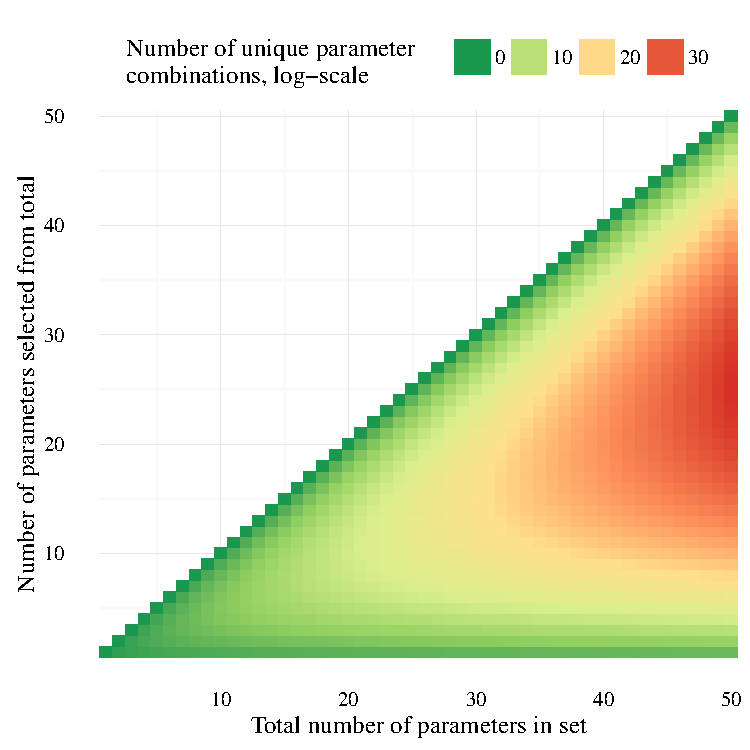
\includegraphics[width=0.6\textwidth]{figs/combnex-1} 

}

\caption[Examples of unique parameter combinations from different parameter sets and number of selected parameters]{Examples of unique parameter combinations from different parameter sets and number of selected parameters.  The number of combinations are shown for increasing numbers of selected parameters from the total in the set, where 50 parameter sets are shown each with one through 50 total parameters. Note that the number of unique combinations is shown as the natural-log.}\label{fig:combnex}
\end{figure}



% effects of changing initial and structural conditions
\begin{figure}[!ht]

{\centering 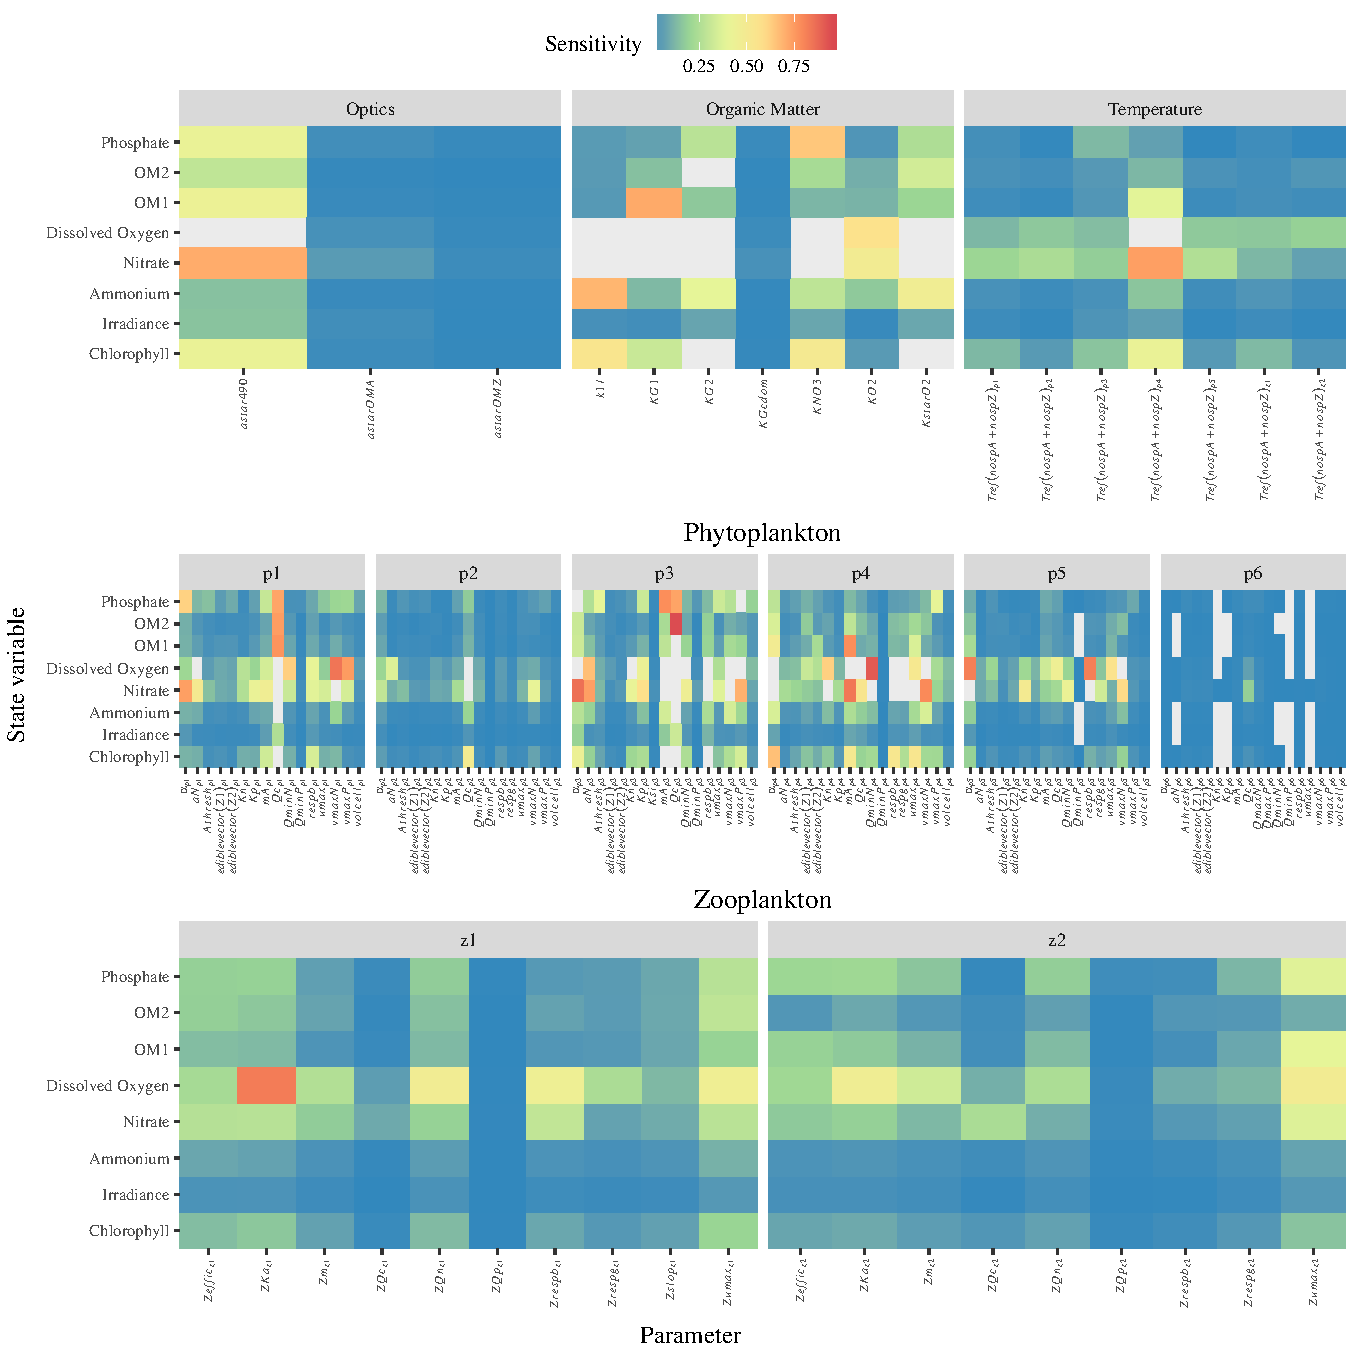
\includegraphics[width=0.7\textwidth]{figs/sensalltile-1} 

}

\caption{Sensitivity values (L1, \cref{l1}) of all state variables to changes in a 50\% increase in parameter values. Parameters are grouped by category: optics, organic matter, phytoplankton, zooplankton, temperature, and zoplankton.  See \cref{tab:dosens} for L1 values for \ac{do} and \cref{tab:nh4sens,tab:chlsens,tab:irrsens,tab:no3sens,tab:om1sens,tab:om2sens,tab:po4sens} for the other state variables.}\label{fig:sensalltile}
\end{figure}



% identifiability plot
\begin{figure}[!ht]

{\centering 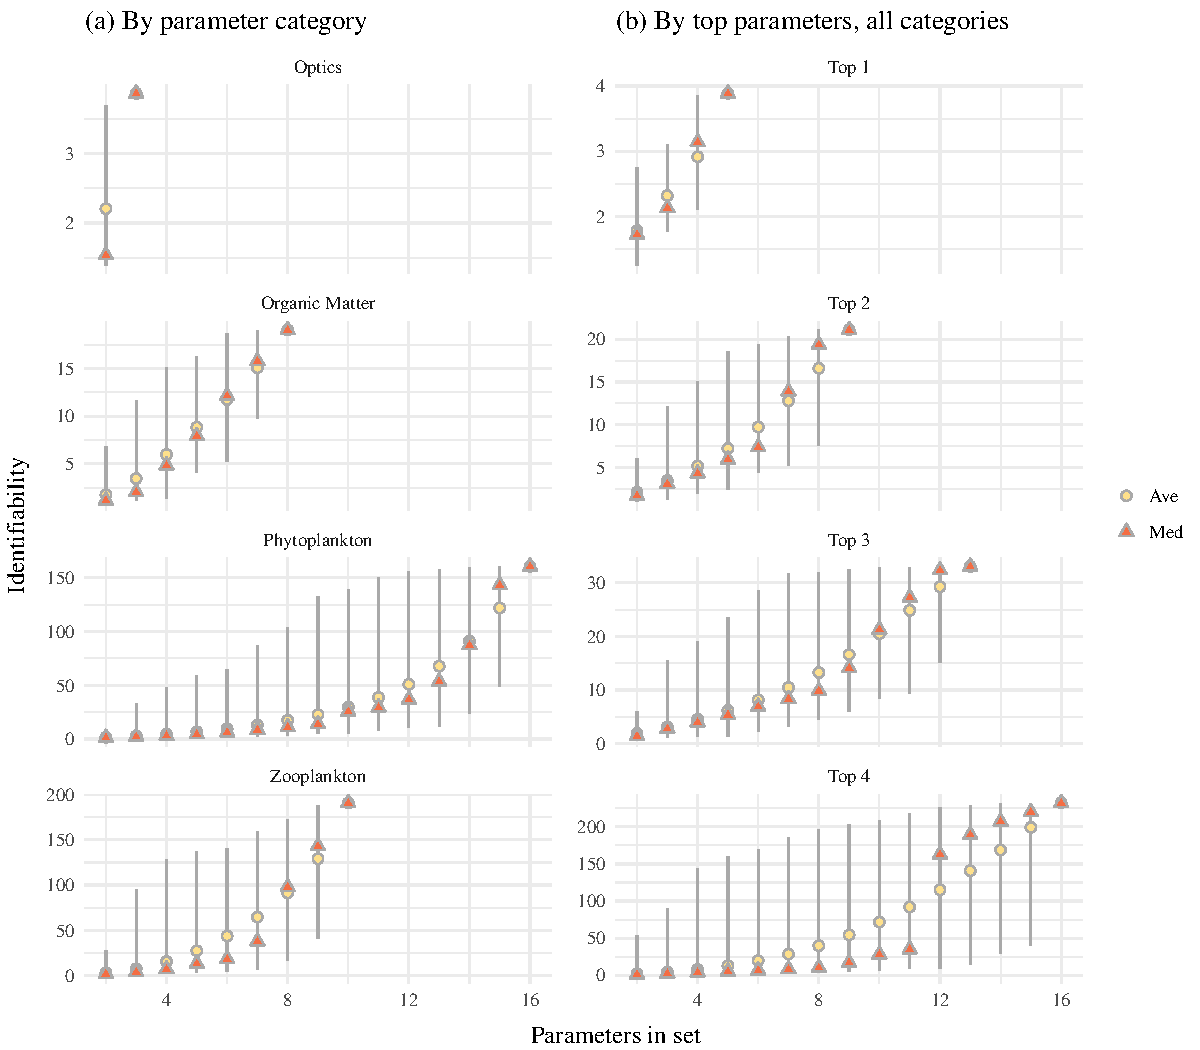
\includegraphics[width=\maxwidth]{figs/identplo-1} 

}

\caption{Identifiability (as $\gamma$, \cref{gameq}) of parameter subsets for \ac{do}.  Plots in (a) show identifiability by parameter categories and (b) shows identifiability by selecting the top 1 through 4 parameters in all categories.  Lines represent identifiability ranges for the possible combinations given the number of parameters in the set.  The temperature category is not shown because \ac{do} was sensitive to only one parameter (i.e., $\gamma = 1$).}\label{fig:identplo}
\end{figure}



% identifiability plot, all state variables
\begin{figure}[!ht]

{\centering 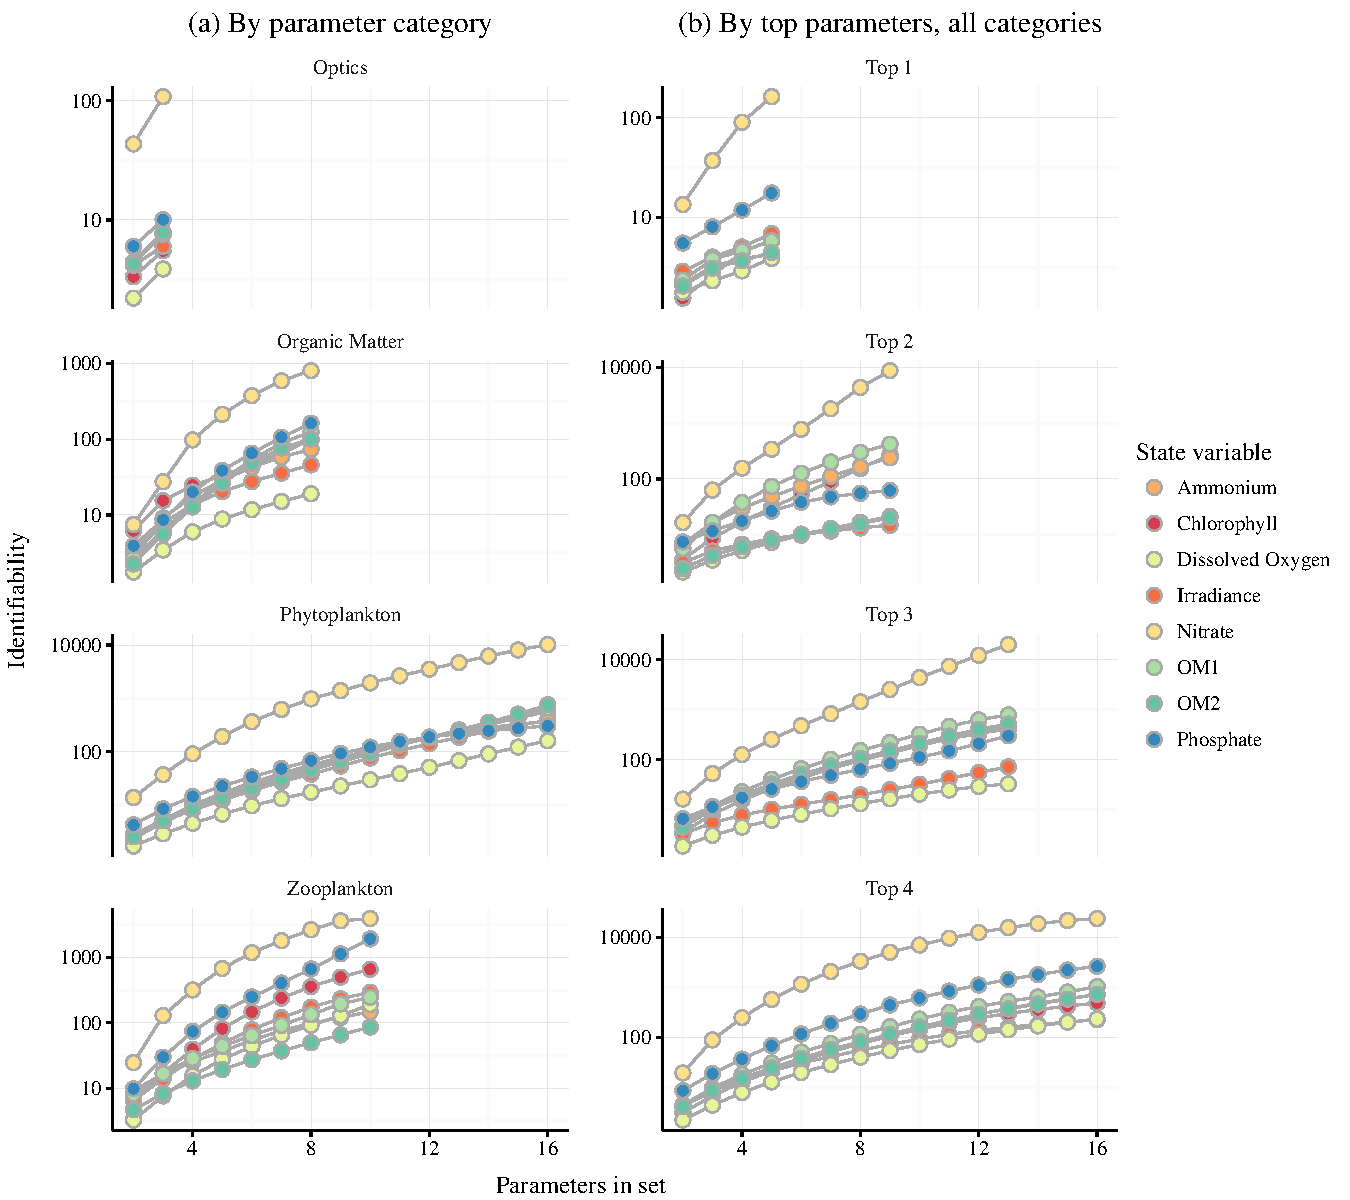
\includegraphics[width=\maxwidth]{figs/identploall-1} 

}

\caption[Average identifiability (as $\gamma$, \cref{gameq}) of parameter subsets for all state variables]{Average identifiability (as $\gamma$, \cref{gameq}) of parameter subsets for all state variables.  Plots in (a) show identifiability by parameter categories and (b) shows identifiability by selecting the top 1 through 4 parameters in all categories.  Identifiability was averaged for all combinations in a parameter set to evaluate relative differenes between state variables.  The temperature category is not shown because all state variables were sensitive to only one parameter (i.e., $\gamma = 1$).}\label{fig:identploall}
\end{figure}



% percent below gamma thresholds
\begin{figure}[!ht]

{\centering 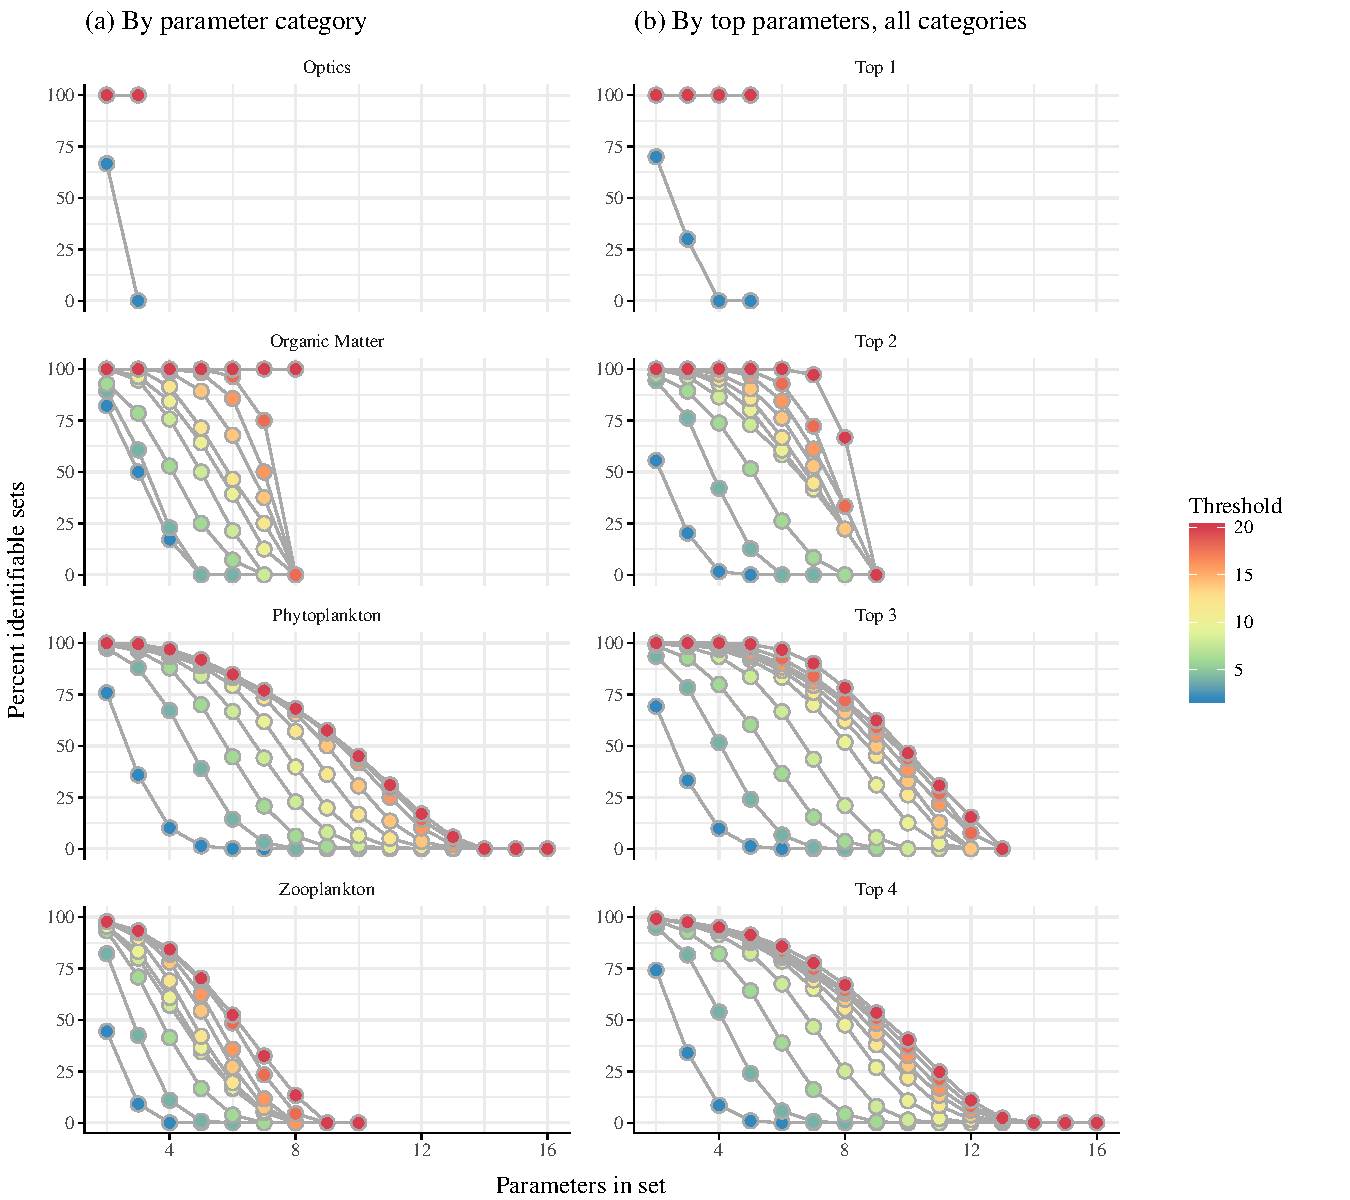
\includegraphics[width=\maxwidth]{figs/percthresh-1} 

}

\caption{Percent of identifiable parameter sets for \ac{do} at different $\gamma$ thresholds, selection criteria, and total number of parameters in the set.  Thresholds varied from $\gamma = 2$ to $20$ such that sets with $\gamma$ below a threshold were considered identifiable relative to the value. Plots in (a) show percent of identifiable sets by selecting parameters within categories and (b) shows percent identifiable by selecting from the top 1 through 4 parameters in all categories.  Percent identifiable was based on all sets in \cref{fig:identplo}.}\label{fig:percthresh}
\end{figure}



% parameter exclusion temp
\begin{figure}[!ht]

{\centering 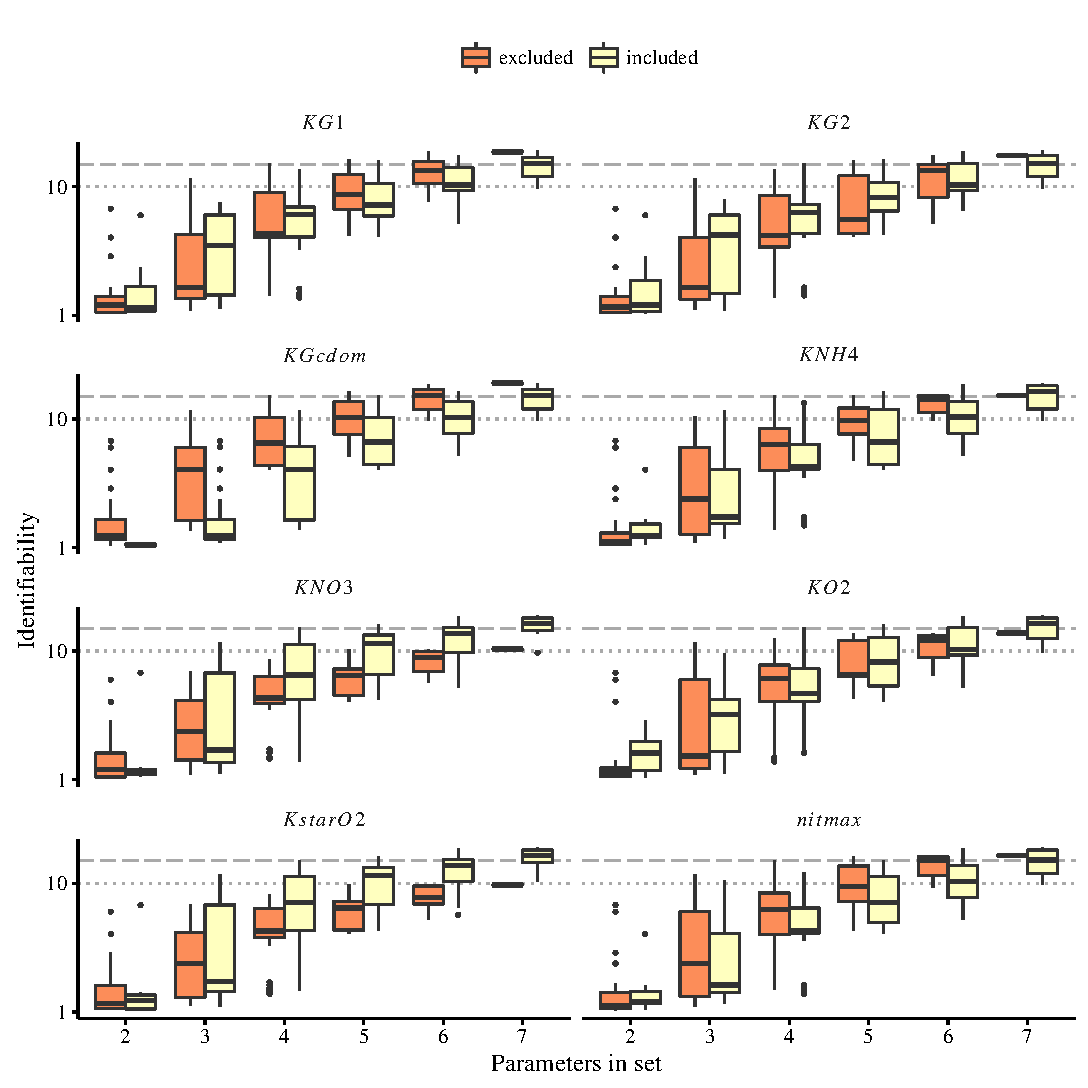
\includegraphics[width=0.8\textwidth]{figs/exclex-1} 

}

\caption{Identifiability (as $\gamma$, \cref{gameq}) for \ac{do} of organic matter parameters for subset combinations in \cref{fig:identplo}.  Identifiability is evaluated for subsets that excluded and included the parameters at the top of each plot. Identifiability of including all eight parameters is in \cref{fig:identplo}. Grey lines indicate potential thresholds at $\gamma = 10, 15$ for maximum acceptable identifiability.}\label{fig:exclex}
\end{figure}



\clearpage

% supplementary material
\beginsupplement

%%
% sup tabs

% ammonium sensitivity all categories
%latex.default(totab, file = "", rowlabel = "Description", caption = cap.val,     caption.loc = "top", rowname = Description, rgroup = unique(cats),     n.rgroup = as.numeric(table(cats)), size = tabsize, label = paste0("tab:",         tablab), insert.bottom = foot.val)%
\begin{table}[!tbp]
{\footnotesize
\caption{Sensitivity of ammonium to perturbations of individual parameters.  Sensitivities are based on a 50\% increase from the initial parameter value, where $L1$ summarizes differences in model output from the default (see \cref{l1}).  Parameters that did not affect ammonium are not shown.  Parameters are grouped by categories as optics, temperature, phytoplankton, zooplankton, and organic matter.\label{tab:nh4sens}} 
\begin{center}
\begin{tabular}{lll}
\hline\hline
\multicolumn{1}{l}{Description}&\multicolumn{1}{c}{Parameter}&\multicolumn{1}{c}{L1}\tabularnewline
\hline
{\bfseries Optics}&&\tabularnewline
~~Chla specific absorption at 490 nm&\textit{astar490}&$0.03$\tabularnewline
~~OMA specific absorption at 490 nm&\textit{astarOMA}&$1.63\times 10^{-3}$\tabularnewline
~~OMZ specific absorption at 490 nm&\textit{astarOMZ}&$1.5\times 10^{-3}$\tabularnewline
\hline
{\bfseries Temperature}&&\tabularnewline
~~Optimum temperature for growth(C)&\textit{Tref(nospA+nospZ)$_{p1}$}&$0.79$\tabularnewline
\hline
{\bfseries Phytoplankton}&&\tabularnewline
~~mortality coefficient&\textit{mA}&$8.49$\tabularnewline
~~edibility vector for Z1&\textit{ediblevector(Z1)}&$1.32$\tabularnewline
~~maximum growth rate&\textit{umax}&$0.65$\tabularnewline
~~initial slope of the photosynthesis-irradiance relationship&\textit{alpha}&$0.6$\tabularnewline
~~N-uptake rate measured at umax&\textit{vmaxN}&$0.46$\tabularnewline
~~Phytoplankton threshold for grazing, is multiplied by VOLcell&\textit{Athresh}&$0.29$\tabularnewline
~~coefficient for non-limiting nutrient&\textit{aN}&$0.17$\tabularnewline
~~phytoplankton growth respiration coefficient&\textit{respg}&$0.16$\tabularnewline
~~phytoplankton basal respiration coefficient&\textit{respb}&$0.15$\tabularnewline
~~half-saturation constant for P&\textit{Kp}&$0.14$\tabularnewline
~~phytoplankton volume/cell&\textit{volcell}&$0.14$\tabularnewline
~~minimum N cell-quota&\textit{QminN}&$0.1$\tabularnewline
~~P-uptake rate measured at umax&\textit{vmaxP}&$0.1$\tabularnewline
~~phytoplankton carbon/cell&\textit{Qc}&$0.03$\tabularnewline
~~half-saturation constant for N&\textit{Kn}&$0.01$\tabularnewline
~~minimum P cell-quota&\textit{QminP}&$2.24\times 10^{-6}$\tabularnewline
\hline
{\bfseries Zooplankton}&&\tabularnewline
~~maximum growth rate of zooplankton&\textit{Zumax}&$1.42$\tabularnewline
~~assimilation efficiency as a fraction of ingestion&\textit{Zeffic}&$0.76$\tabularnewline
~~half saturation coefficient for grazing&\textit{ZKa}&$0.74$\tabularnewline
~~zooplankton nitrogen/individual&\textit{ZQn}&$0.62$\tabularnewline
~~Zooplankton mortality constant for quadratic mortality&\textit{Zm}&$0.5$\tabularnewline
~~proportion of grazed phytoplankton lost to sloppy feeding&\textit{Zslop}&$0.3$\tabularnewline
~~Zooplankton growth-dependent respiration factor&\textit{Zrespg}&$0.22$\tabularnewline
~~Zooplankton biomass-dependent respiration factor&\textit{Zrespb}&$0.16$\tabularnewline
~~zooplankton phosphorus/individual&\textit{ZQp}&$1.07\times 10^{-3}$\tabularnewline
~~zooplankton carbon/individual&\textit{ZQc}&$1.44\times 10^{-4}$\tabularnewline
\hline
{\bfseries Organic Matter}&&\tabularnewline
~~maximum rate of nitrification per day&\textit{nitmax}&$1.54$\tabularnewline
~~NH4 rate constant for nitrification&\textit{KNH4}&$0.66$\tabularnewline
~~turnover rate for OM1A and OM1Z&\textit{KG1}&$0.07$\tabularnewline
~~decay rate of CDOM, 1/day&\textit{KGcdom}&$0.07$\tabularnewline
~~half-saturation concentration for O2 utilization&\textit{KO2}&$0.06$\tabularnewline
~~O2 concentration that inhibits denitrification&\textit{KstarO2}&$0.05$\tabularnewline
~~turnover rate for OM2A and OM2Z&\textit{KG2}&$0.03$\tabularnewline
~~half-saturation concentration for NO3 used in denitrification&\textit{KNO3}&$7.55\times 10^{-3}$\tabularnewline
\hline
\end{tabular}\end{center}}
\end{table}


% chlorophyll sensitivity all categories
%latex.default(totab, file = "", rowlabel = "Description", caption = cap.val,     caption.loc = "top", rowname = Description, rgroup = unique(cats),     n.rgroup = as.numeric(table(cats)), size = tabsize, label = paste0("tab:",         tablab), insert.bottom = foot.val)%
\begin{table}[!tbp]
{\footnotesize
\caption{Sensitivity of \ac{chla} to perturbations of individual parameters.  Sensitivities are based on a 50\% increase from the initial parameter value, where $L1$ summarizes differences in model output from the default (see \cref{l1}).  Parameters that did not affect \ac{chla} are not shown.  Parameters are grouped by categories as optics, temperature, phytoplankton, zooplankton, and organic matter.\label{tab:chlsens}} 
\begin{center}
\begin{tabular}{lll}
\hline\hline
\multicolumn{1}{l}{Description}&\multicolumn{1}{c}{Parameter}&\multicolumn{1}{c}{L1}\tabularnewline
\hline
{\bfseries Optics}&&\tabularnewline
~~Chla specific absorption at 490 nm&\textit{astar490}&$0.02$\tabularnewline
~~OMA specific absorption at 490 nm&\textit{astarOMA}&$1.45\times 10^{-3}$\tabularnewline
~~OMZ specific absorption at 490 nm&\textit{astarOMZ}&$1.13\times 10^{-3}$\tabularnewline
\hline
{\bfseries Temperature}&&\tabularnewline
~~Optimum temperature for growth(C)&\textit{Tref(nospA+nospZ)$_{p1}$}&$0.6$\tabularnewline
\hline
{\bfseries Phytoplankton}&&\tabularnewline
~~mortality coefficient&\textit{mA}&$13.94$\tabularnewline
~~edibility vector for Z1&\textit{ediblevector(Z1)}&$0.95$\tabularnewline
~~maximum growth rate&\textit{umax}&$0.85$\tabularnewline
~~initial slope of the photosynthesis-irradiance relationship&\textit{alpha}&$0.62$\tabularnewline
~~N-uptake rate measured at umax&\textit{vmaxN}&$0.53$\tabularnewline
~~phytoplankton growth respiration coefficient&\textit{respg}&$0.26$\tabularnewline
~~Phytoplankton threshold for grazing, is multiplied by VOLcell&\textit{Athresh}&$0.25$\tabularnewline
~~phytoplankton basal respiration coefficient&\textit{respb}&$0.24$\tabularnewline
~~coefficient for non-limiting nutrient&\textit{aN}&$0.17$\tabularnewline
~~half-saturation constant for P&\textit{Kp}&$0.14$\tabularnewline
~~P-uptake rate measured at umax&\textit{vmaxP}&$0.12$\tabularnewline
~~phytoplankton volume/cell&\textit{volcell}&$0.1$\tabularnewline
~~minimum N cell-quota&\textit{QminN}&$0.07$\tabularnewline
~~phytoplankton carbon/cell&\textit{Qc}&$0.02$\tabularnewline
~~half-saturation constant for N&\textit{Kn}&$0.01$\tabularnewline
~~minimum P cell-quota&\textit{QminP}&$1.38\times 10^{-6}$\tabularnewline
\hline
{\bfseries Zooplankton}&&\tabularnewline
~~maximum growth rate of zooplankton&\textit{Zumax}&$1.02$\tabularnewline
~~half saturation coefficient for grazing&\textit{ZKa}&$0.85$\tabularnewline
~~assimilation efficiency as a fraction of ingestion&\textit{Zeffic}&$0.57$\tabularnewline
~~zooplankton nitrogen/individual&\textit{ZQn}&$0.52$\tabularnewline
~~Zooplankton mortality constant for quadratic mortality&\textit{Zm}&$0.41$\tabularnewline
~~proportion of grazed phytoplankton lost to sloppy feeding&\textit{Zslop}&$0.23$\tabularnewline
~~Zooplankton growth-dependent respiration factor&\textit{Zrespg}&$0.17$\tabularnewline
~~Zooplankton biomass-dependent respiration factor&\textit{Zrespb}&$0.14$\tabularnewline
~~zooplankton phosphorus/individual&\textit{ZQp}&$1.29\times 10^{-3}$\tabularnewline
~~zooplankton carbon/individual&\textit{ZQc}&$7.55\times 10^{-5}$\tabularnewline
\hline
{\bfseries Organic Matter}&&\tabularnewline
~~decay rate of CDOM, 1/day&\textit{KGcdom}&$0.07$\tabularnewline
~~turnover rate for OM1A and OM1Z&\textit{KG1}&$0.03$\tabularnewline
~~turnover rate for OM2A and OM2Z&\textit{KG2}&$0.01$\tabularnewline
~~O2 concentration that inhibits denitrification&\textit{KstarO2}&$0.01$\tabularnewline
~~half-saturation concentration for O2 utilization&\textit{KO2}&$3.35\times 10^{-3}$\tabularnewline
~~half-saturation concentration for NO3 used in denitrification&\textit{KNO3}&$1.19\times 10^{-3}$\tabularnewline
~~maximum rate of nitrification per day&\textit{nitmax}&$3.4\times 10^{-5}$\tabularnewline
~~NH4 rate constant for nitrification&\textit{KNH4}&$2.97\times 10^{-5}$\tabularnewline
\hline
\end{tabular}\end{center}}
\end{table}


% irradiance sensitivity all categories
%latex.default(totab, file = "", rowlabel = "Description", caption = cap.val,     caption.loc = "top", rowname = Description, rgroup = unique(cats),     n.rgroup = as.numeric(table(cats)), size = tabsize, label = paste0("tab:",         tablab), insert.bottom = foot.val)%
\begin{table}[!tbp]
{\footnotesize
\caption{Sensitivity of irradiance to perturbations of individual parameters.  Sensitivities are based on a 50\% increase from the initial parameter value, where $L1$ summarizes differences in model output from the default (see \cref{l1}).  Parameters that did not affect irradiance are not shown.  Parameters are grouped by categories as optics, temperature, phytoplankton, zooplankton, and organic matter.\label{tab:irrsens}} 
\begin{center}
\begin{tabular}{lll}
\hline\hline
\multicolumn{1}{l}{Description}&\multicolumn{1}{c}{Parameter}&\multicolumn{1}{c}{L1}\tabularnewline
\hline
{\bfseries Optics}&&\tabularnewline
~~Chla specific absorption at 490 nm&\textit{astar490}&$0.02$\tabularnewline
~~OMA specific absorption at 490 nm&\textit{astarOMA}&$1.47\times 10^{-3}$\tabularnewline
~~OMZ specific absorption at 490 nm&\textit{astarOMZ}&$1.34\times 10^{-3}$\tabularnewline
\hline
{\bfseries Temperature}&&\tabularnewline
~~Optimum temperature for growth(C)&\textit{Tref(nospA+nospZ)$_{p1}$}&$0.03$\tabularnewline
\hline
{\bfseries Phytoplankton}&&\tabularnewline
~~maximum growth rate&\textit{umax}&$0.09$\tabularnewline
~~mortality coefficient&\textit{mA}&$0.05$\tabularnewline
~~initial slope of the photosynthesis-irradiance relationship&\textit{alpha}&$0.04$\tabularnewline
~~edibility vector for Z1&\textit{ediblevector(Z1)}&$0.04$\tabularnewline
~~N-uptake rate measured at umax&\textit{vmaxN}&$0.03$\tabularnewline
~~Phytoplankton threshold for grazing, is multiplied by VOLcell&\textit{Athresh}&$0.02$\tabularnewline
~~coefficient for non-limiting nutrient&\textit{aN}&$0.01$\tabularnewline
~~phytoplankton growth respiration coefficient&\textit{respg}&$0.01$\tabularnewline
~~half-saturation constant for P&\textit{Kp}&$0.01$\tabularnewline
~~P-uptake rate measured at umax&\textit{vmaxP}&$9.48\times 10^{-3}$\tabularnewline
~~phytoplankton basal respiration coefficient&\textit{respb}&$9.38\times 10^{-3}$\tabularnewline
~~phytoplankton volume/cell&\textit{volcell}&$8.1\times 10^{-3}$\tabularnewline
~~minimum N cell-quota&\textit{QminN}&$5.75\times 10^{-3}$\tabularnewline
~~phytoplankton carbon/cell&\textit{Qc}&$3.78\times 10^{-3}$\tabularnewline
~~half-saturation constant for N&\textit{Kn}&$9.81\times 10^{-4}$\tabularnewline
~~minimum P cell-quota&\textit{QminP}&$1.92\times 10^{-7}$\tabularnewline
\hline
{\bfseries Zooplankton}&&\tabularnewline
~~half saturation coefficient for grazing&\textit{ZKa}&$0.13$\tabularnewline
~~zooplankton nitrogen/individual&\textit{ZQn}&$0.06$\tabularnewline
~~maximum growth rate of zooplankton&\textit{Zumax}&$0.04$\tabularnewline
~~Zooplankton mortality constant for quadratic mortality&\textit{Zm}&$0.04$\tabularnewline
~~assimilation efficiency as a fraction of ingestion&\textit{Zeffic}&$0.03$\tabularnewline
~~proportion of grazed phytoplankton lost to sloppy feeding&\textit{Zslop}&$0.02$\tabularnewline
~~Zooplankton growth-dependent respiration factor&\textit{Zrespg}&$0.01$\tabularnewline
~~Zooplankton biomass-dependent respiration factor&\textit{Zrespb}&$9.67\times 10^{-3}$\tabularnewline
~~zooplankton phosphorus/individual&\textit{ZQp}&$9.34\times 10^{-5}$\tabularnewline
~~zooplankton carbon/individual&\textit{ZQc}&$1.99\times 10^{-5}$\tabularnewline
\hline
{\bfseries Organic Matter}&&\tabularnewline
~~decay rate of CDOM, 1/day&\textit{KGcdom}&$0.05$\tabularnewline
~~turnover rate for OM1A and OM1Z&\textit{KG1}&$3.96\times 10^{-3}$\tabularnewline
~~turnover rate for OM2A and OM2Z&\textit{KG2}&$9.88\times 10^{-4}$\tabularnewline
~~O2 concentration that inhibits denitrification&\textit{KstarO2}&$7.2\times 10^{-4}$\tabularnewline
~~half-saturation concentration for O2 utilization&\textit{KO2}&$3.54\times 10^{-4}$\tabularnewline
~~half-saturation concentration for NO3 used in denitrification&\textit{KNO3}&$6.18\times 10^{-5}$\tabularnewline
~~maximum rate of nitrification per day&\textit{nitmax}&$1.72\times 10^{-6}$\tabularnewline
~~NH4 rate constant for nitrification&\textit{KNH4}&$1.48\times 10^{-6}$\tabularnewline
\hline
\end{tabular}\end{center}}
\end{table}


% nitrate sensitivity all categories
%latex.default(totab, file = "", rowlabel = "Description", caption = cap.val,     caption.loc = "top", rowname = Description, rgroup = unique(cats),     n.rgroup = as.numeric(table(cats)), size = tabsize, label = paste0("tab:",         tablab), insert.bottom = foot.val)%
\begin{table}[!tbp]
{\footnotesize
\caption{Sensitivity of nitrate to perturbations of individual parameters.  Sensitivities are based on a 50\% increase from the initial parameter value, where $L1$ summarizes differences in model output from the default (see \cref{l1}).  Parameters that did not affect nitrate are not shown.  Parameters are grouped by categories as optics, temperature, phytoplankton, zooplankton, and organic matter.\label{tab:no3sens}} 
\begin{center}
\begin{tabular}{lll}
\hline\hline
\multicolumn{1}{l}{Description}&\multicolumn{1}{c}{Parameter}&\multicolumn{1}{c}{L1}\tabularnewline
\hline
{\bfseries Optics}&&\tabularnewline
~~Chla specific absorption at 490 nm&\textit{astar490}&$0.02$\tabularnewline
~~OMZ specific absorption at 490 nm&\textit{astarOMZ}&$1.27\times 10^{-3}$\tabularnewline
~~OMA specific absorption at 490 nm&\textit{astarOMA}&$1.19\times 10^{-3}$\tabularnewline
\hline
{\bfseries Temperature}&&\tabularnewline
~~Optimum temperature for growth(C)&\textit{Tref(nospA+nospZ)$_{p1}$}&$0.3$\tabularnewline
\hline
{\bfseries Phytoplankton}&&\tabularnewline
~~maximum growth rate&\textit{umax}&$8.49$\tabularnewline
~~phytoplankton carbon/cell&\textit{Qc}&$0.89$\tabularnewline
~~initial slope of the photosynthesis-irradiance relationship&\textit{alpha}&$0.7$\tabularnewline
~~edibility vector for Z1&\textit{ediblevector(Z1)}&$0.33$\tabularnewline
~~mortality coefficient&\textit{mA}&$0.27$\tabularnewline
~~Phytoplankton threshold for grazing, is multiplied by VOLcell&\textit{Athresh}&$0.2$\tabularnewline
~~N-uptake rate measured at umax&\textit{vmaxN}&$0.19$\tabularnewline
~~coefficient for non-limiting nutrient&\textit{aN}&$0.13$\tabularnewline
~~phytoplankton growth respiration coefficient&\textit{respg}&$0.11$\tabularnewline
~~phytoplankton volume/cell&\textit{volcell}&$0.1$\tabularnewline
~~P-uptake rate measured at umax&\textit{vmaxP}&$0.1$\tabularnewline
~~half-saturation constant for P&\textit{Kp}&$0.09$\tabularnewline
~~minimum N cell-quota&\textit{QminN}&$0.09$\tabularnewline
~~phytoplankton basal respiration coefficient&\textit{respb}&$0.07$\tabularnewline
~~half-saturation constant for N&\textit{Kn}&$7.06\times 10^{-3}$\tabularnewline
~~minimum P cell-quota&\textit{QminP}&$6.67\times 10^{-7}$\tabularnewline
\hline
{\bfseries Zooplankton}&&\tabularnewline
~~half saturation coefficient for grazing&\textit{ZKa}&$7.59$\tabularnewline
~~zooplankton nitrogen/individual&\textit{ZQn}&$1.17$\tabularnewline
~~Zooplankton mortality constant for quadratic mortality&\textit{Zm}&$0.7$\tabularnewline
~~maximum growth rate of zooplankton&\textit{Zumax}&$0.34$\tabularnewline
~~proportion of grazed phytoplankton lost to sloppy feeding&\textit{Zslop}&$0.26$\tabularnewline
~~assimilation efficiency as a fraction of ingestion&\textit{Zeffic}&$0.25$\tabularnewline
~~Zooplankton growth-dependent respiration factor&\textit{Zrespg}&$0.17$\tabularnewline
~~Zooplankton biomass-dependent respiration factor&\textit{Zrespb}&$0.1$\tabularnewline
~~zooplankton carbon/individual&\textit{ZQc}&$3.8\times 10^{-3}$\tabularnewline
~~zooplankton phosphorus/individual&\textit{ZQp}&$8.59\times 10^{-4}$\tabularnewline
\hline
{\bfseries Organic Matter}&&\tabularnewline
~~O2 concentration that inhibits denitrification&\textit{KstarO2}&$0.78$\tabularnewline
~~half-saturation concentration for NO3 used in denitrification&\textit{KNO3}&$0.07$\tabularnewline
~~decay rate of CDOM, 1/day&\textit{KGcdom}&$0.04$\tabularnewline
~~half-saturation concentration for O2 utilization&\textit{KO2}&$0.03$\tabularnewline
~~turnover rate for OM1A and OM1Z&\textit{KG1}&$0.02$\tabularnewline
~~turnover rate for OM2A and OM2Z&\textit{KG2}&$0.01$\tabularnewline
~~maximum rate of nitrification per day&\textit{nitmax}&$9.96\times 10^{-3}$\tabularnewline
~~NH4 rate constant for nitrification&\textit{KNH4}&$9.87\times 10^{-3}$\tabularnewline
\hline
\end{tabular}\end{center}}
\end{table}


% om1 sensitivity all categories
%latex.default(totab, file = "", rowlabel = "Description", caption = cap.val,     caption.loc = "top", rowname = Description, rgroup = unique(cats),     n.rgroup = as.numeric(table(cats)), size = tabsize, label = paste0("tab:",         tablab), insert.bottom = foot.val)%
\begin{table}[!tbp]
{\footnotesize
\caption{Sensitivity of \ac{pom} to perturbations of individual parameters.  Sensitivities are based on a 50\% increase from the initial parameter value, where $L1$ summarizes differences in model output from the default (see \cref{l1}).  Parameters that did not affect \ac{pom} are not shown.  Parameters are grouped by categories as optics, temperature, phytoplankton, zooplankton, and organic matter.\label{tab:om1sens}} 
\begin{center}
\begin{tabular}{lll}
\hline\hline
\multicolumn{1}{l}{Description}&\multicolumn{1}{c}{Parameter}&\multicolumn{1}{c}{L1}\tabularnewline
\hline
{\bfseries Optics}&&\tabularnewline
~~Chla specific absorption at 490 nm&\textit{astar490}&$0.03$\tabularnewline
~~OMA specific absorption at 490 nm&\textit{astarOMA}&$1.73\times 10^{-3}$\tabularnewline
~~OMZ specific absorption at 490 nm&\textit{astarOMZ}&$1.49\times 10^{-3}$\tabularnewline
\hline
{\bfseries Temperature}&&\tabularnewline
~~Optimum temperature for growth(C)&\textit{Tref(nospA+nospZ)$_{p1}$}&$0.86$\tabularnewline
\hline
{\bfseries Phytoplankton}&&\tabularnewline
~~mortality coefficient&\textit{mA}&$7.22$\tabularnewline
~~edibility vector for Z1&\textit{ediblevector(Z1)}&$0.9$\tabularnewline
~~maximum growth rate&\textit{umax}&$0.89$\tabularnewline
~~phytoplankton carbon/cell&\textit{Qc}&$0.67$\tabularnewline
~~initial slope of the photosynthesis-irradiance relationship&\textit{alpha}&$0.67$\tabularnewline
~~N-uptake rate measured at umax&\textit{vmaxN}&$0.45$\tabularnewline
~~phytoplankton growth respiration coefficient&\textit{respg}&$0.29$\tabularnewline
~~phytoplankton basal respiration coefficient&\textit{respb}&$0.24$\tabularnewline
~~Phytoplankton threshold for grazing, is multiplied by VOLcell&\textit{Athresh}&$0.22$\tabularnewline
~~minimum N cell-quota&\textit{QminN}&$0.21$\tabularnewline
~~coefficient for non-limiting nutrient&\textit{aN}&$0.14$\tabularnewline
~~half-saturation constant for P&\textit{Kp}&$0.11$\tabularnewline
~~phytoplankton volume/cell&\textit{volcell}&$0.1$\tabularnewline
~~P-uptake rate measured at umax&\textit{vmaxP}&$0.09$\tabularnewline
~~half-saturation constant for N&\textit{Kn}&$0.01$\tabularnewline
~~minimum P cell-quota&\textit{QminP}&$7.35\times 10^{-4}$\tabularnewline
\hline
{\bfseries Zooplankton}&&\tabularnewline
~~maximum growth rate of zooplankton&\textit{Zumax}&$0.96$\tabularnewline
~~half saturation coefficient for grazing&\textit{ZKa}&$0.79$\tabularnewline
~~assimilation efficiency as a fraction of ingestion&\textit{Zeffic}&$0.54$\tabularnewline
~~zooplankton nitrogen/individual&\textit{ZQn}&$0.49$\tabularnewline
~~Zooplankton mortality constant for quadratic mortality&\textit{Zm}&$0.39$\tabularnewline
~~proportion of grazed phytoplankton lost to sloppy feeding&\textit{Zslop}&$0.27$\tabularnewline
~~Zooplankton growth-dependent respiration factor&\textit{Zrespg}&$0.16$\tabularnewline
~~Zooplankton biomass-dependent respiration factor&\textit{Zrespb}&$0.12$\tabularnewline
~~zooplankton carbon/individual&\textit{ZQc}&$9.64\times 10^{-3}$\tabularnewline
~~zooplankton phosphorus/individual&\textit{ZQp}&$1.06\times 10^{-3}$\tabularnewline
\hline
{\bfseries Organic Matter}&&\tabularnewline
~~turnover rate for OM1A and OM1Z&\textit{KG1}&$0.92$\tabularnewline
~~decay rate of CDOM, 1/day&\textit{KGcdom}&$0.07$\tabularnewline
~~half-saturation concentration for O2 utilization&\textit{KO2}&$0.04$\tabularnewline
~~O2 concentration that inhibits denitrification&\textit{KstarO2}&$0.02$\tabularnewline
~~turnover rate for OM2A and OM2Z&\textit{KG2}&$0.01$\tabularnewline
~~half-saturation concentration for NO3 used in denitrification&\textit{KNO3}&$3.72\times 10^{-3}$\tabularnewline
~~maximum rate of nitrification per day&\textit{nitmax}&$6.98\times 10^{-5}$\tabularnewline
~~NH4 rate constant for nitrification&\textit{KNH4}&$6.41\times 10^{-5}$\tabularnewline
\hline
\end{tabular}\end{center}}
\end{table}


% om2 sensitivity all categories
%latex.default(totab, file = "", rowlabel = "Description", caption = cap.val,     caption.loc = "top", rowname = Description, rgroup = unique(cats),     n.rgroup = as.numeric(table(cats)), size = tabsize, label = paste0("tab:",         tablab), insert.bottom = foot.val)%
\begin{table}[!tbp]
{\footnotesize
\caption{Sensitivity of \acl{dom} to perturbations of individual parameters.  Sensitivities are based on a 50\% increase from the initial parameter value, where $L1$ summarizes differences in model output from the default (see \cref{l1}).  Parameters that did not affect \acl{dom} are not shown.  Parameters are grouped by categories as optics, temperature, phytoplankton, zooplankton, and organic matter.\label{tab:om2sens}} 
\begin{center}
\begin{tabular}{lll}
\hline\hline
\multicolumn{1}{l}{Description}&\multicolumn{1}{c}{Parameter}&\multicolumn{1}{c}{L1}\tabularnewline
\hline
{\bfseries Optics}&&\tabularnewline
~~Chla specific absorption at 490 nm&\textit{astar490}&$0.04$\tabularnewline
~~OMA specific absorption at 490 nm&\textit{astarOMA}&$2.48\times 10^{-3}$\tabularnewline
~~OMZ specific absorption at 490 nm&\textit{astarOMZ}&$2.04\times 10^{-3}$\tabularnewline
\hline
{\bfseries Temperature}&&\tabularnewline
~~Optimum temperature for growth(C)&\textit{Tref(nospA+nospZ)$_{p1}$}&$1.48$\tabularnewline
\hline
{\bfseries Phytoplankton}&&\tabularnewline
~~mortality coefficient&\textit{mA}&$14.25$\tabularnewline
~~maximum growth rate&\textit{umax}&$1.11$\tabularnewline
~~edibility vector for Z1&\textit{ediblevector(Z1)}&$0.94$\tabularnewline
~~N-uptake rate measured at umax&\textit{vmaxN}&$0.86$\tabularnewline
~~initial slope of the photosynthesis-irradiance relationship&\textit{alpha}&$0.85$\tabularnewline
~~phytoplankton carbon/cell&\textit{Qc}&$0.67$\tabularnewline
~~phytoplankton growth respiration coefficient&\textit{respg}&$0.36$\tabularnewline
~~phytoplankton basal respiration coefficient&\textit{respb}&$0.29$\tabularnewline
~~coefficient for non-limiting nutrient&\textit{aN}&$0.25$\tabularnewline
~~minimum N cell-quota&\textit{QminN}&$0.24$\tabularnewline
~~Phytoplankton threshold for grazing, is multiplied by VOLcell&\textit{Athresh}&$0.22$\tabularnewline
~~half-saturation constant for P&\textit{Kp}&$0.2$\tabularnewline
~~P-uptake rate measured at umax&\textit{vmaxP}&$0.14$\tabularnewline
~~phytoplankton volume/cell&\textit{volcell}&$0.1$\tabularnewline
~~half-saturation constant for N&\textit{Kn}&$0.02$\tabularnewline
~~minimum P cell-quota&\textit{QminP}&$4.37\times 10^{-3}$\tabularnewline
\hline
{\bfseries Zooplankton}&&\tabularnewline
~~maximum growth rate of zooplankton&\textit{Zumax}&$1.01$\tabularnewline
~~half saturation coefficient for grazing&\textit{ZKa}&$0.88$\tabularnewline
~~assimilation efficiency as a fraction of ingestion&\textit{Zeffic}&$0.58$\tabularnewline
~~zooplankton nitrogen/individual&\textit{ZQn}&$0.54$\tabularnewline
~~Zooplankton mortality constant for quadratic mortality&\textit{Zm}&$0.41$\tabularnewline
~~Zooplankton growth-dependent respiration factor&\textit{Zrespg}&$0.17$\tabularnewline
~~Zooplankton biomass-dependent respiration factor&\textit{Zrespb}&$0.13$\tabularnewline
~~proportion of grazed phytoplankton lost to sloppy feeding&\textit{Zslop}&$0.12$\tabularnewline
~~zooplankton carbon/individual&\textit{ZQc}&$0.04$\tabularnewline
~~zooplankton phosphorus/individual&\textit{ZQp}&$1.69\times 10^{-3}$\tabularnewline
\hline
{\bfseries Organic Matter}&&\tabularnewline
~~turnover rate for OM2A and OM2Z&\textit{KG2}&$0.94$\tabularnewline
~~decay rate of CDOM, 1/day&\textit{KGcdom}&$0.1$\tabularnewline
~~half-saturation concentration for O2 utilization&\textit{KO2}&$0.04$\tabularnewline
~~turnover rate for OM1A and OM1Z&\textit{KG1}&$0.04$\tabularnewline
~~O2 concentration that inhibits denitrification&\textit{KstarO2}&$0.03$\tabularnewline
~~half-saturation concentration for NO3 used in denitrification&\textit{KNO3}&$3.16\times 10^{-3}$\tabularnewline
~~maximum rate of nitrification per day&\textit{nitmax}&$8.44\times 10^{-5}$\tabularnewline
~~NH4 rate constant for nitrification&\textit{KNH4}&$7.41\times 10^{-5}$\tabularnewline
\hline
\end{tabular}\end{center}}
\end{table}


% phosphate sensitivity all categories
%latex.default(totab, file = "", rowlabel = "Description", caption = cap.val,     caption.loc = "top", rowname = Description, rgroup = unique(cats),     n.rgroup = as.numeric(table(cats)), size = tabsize, label = paste0("tab:",         tablab), insert.bottom = foot.val)%
\begin{table}[!tbp]
{\footnotesize
\caption{Sensitivity of phosphate to perturbations of individual parameters.  Sensitivities are based on a 50\% increase from the initial parameter value, where $L1$ summarizes differences in model output from the default (see \cref{l1}).  Parameters that did not affect phosphate are not shown.  Parameters are grouped by categories as optics, temperature, phytoplankton, zooplankton, and organic matter.\label{tab:po4sens}} 
\begin{center}
\begin{tabular}{lll}
\hline\hline
\multicolumn{1}{l}{Description}&\multicolumn{1}{c}{Parameter}&\multicolumn{1}{c}{L1}\tabularnewline
\hline
{\bfseries Optics}&&\tabularnewline
~~Chla specific absorption at 490 nm&\textit{astar490}&$9.01\times 10^{-3}$\tabularnewline
~~OMZ specific absorption at 490 nm&\textit{astarOMZ}&$5.21\times 10^{-4}$\tabularnewline
~~OMA specific absorption at 490 nm&\textit{astarOMA}&$5.13\times 10^{-4}$\tabularnewline
\hline
{\bfseries Temperature}&&\tabularnewline
~~Optimum temperature for growth(C)&\textit{Tref(nospA+nospZ)$_{p1}$}&$0.16$\tabularnewline
\hline
{\bfseries Phytoplankton}&&\tabularnewline
~~maximum growth rate&\textit{umax}&$0.78$\tabularnewline
~~P-uptake rate measured at umax&\textit{vmaxP}&$0.59$\tabularnewline
~~edibility vector for Z1&\textit{ediblevector(Z1)}&$0.25$\tabularnewline
~~initial slope of the photosynthesis-irradiance relationship&\textit{alpha}&$0.23$\tabularnewline
~~mortality coefficient&\textit{mA}&$0.2$\tabularnewline
~~N-uptake rate measured at umax&\textit{vmaxN}&$0.18$\tabularnewline
~~Phytoplankton threshold for grazing, is multiplied by VOLcell&\textit{Athresh}&$0.13$\tabularnewline
~~coefficient for non-limiting nutrient&\textit{aN}&$0.11$\tabularnewline
~~phytoplankton growth respiration coefficient&\textit{respg}&$0.09$\tabularnewline
~~phytoplankton volume/cell&\textit{volcell}&$0.06$\tabularnewline
~~phytoplankton basal respiration coefficient&\textit{respb}&$0.06$\tabularnewline
~~minimum N cell-quota&\textit{QminN}&$0.04$\tabularnewline
~~half-saturation constant for P&\textit{Kp}&$0.03$\tabularnewline
~~half-saturation constant for N&\textit{Kn}&$6.97\times 10^{-3}$\tabularnewline
~~phytoplankton carbon/cell&\textit{Qc}&$6.68\times 10^{-3}$\tabularnewline
~~minimum P cell-quota&\textit{QminP}&$8.21\times 10^{-7}$\tabularnewline
\hline
{\bfseries Zooplankton}&&\tabularnewline
~~half saturation coefficient for grazing&\textit{ZKa}&$1.47$\tabularnewline
~~zooplankton nitrogen/individual&\textit{ZQn}&$0.5$\tabularnewline
~~Zooplankton mortality constant for quadratic mortality&\textit{Zm}&$0.35$\tabularnewline
~~maximum growth rate of zooplankton&\textit{Zumax}&$0.26$\tabularnewline
~~assimilation efficiency as a fraction of ingestion&\textit{Zeffic}&$0.19$\tabularnewline
~~proportion of grazed phytoplankton lost to sloppy feeding&\textit{Zslop}&$0.15$\tabularnewline
~~Zooplankton growth-dependent respiration factor&\textit{Zrespg}&$0.1$\tabularnewline
~~Zooplankton biomass-dependent respiration factor&\textit{Zrespb}&$0.06$\tabularnewline
~~zooplankton phosphorus/individual&\textit{ZQp}&$6.43\times 10^{-3}$\tabularnewline
~~zooplankton carbon/individual&\textit{ZQc}&$3.38\times 10^{-5}$\tabularnewline
\hline
{\bfseries Organic Matter}&&\tabularnewline
~~turnover rate for OM1A and OM1Z&\textit{KG1}&$0.14$\tabularnewline
~~turnover rate for OM2A and OM2Z&\textit{KG2}&$0.06$\tabularnewline
~~decay rate of CDOM, 1/day&\textit{KGcdom}&$0.02$\tabularnewline
~~half-saturation concentration for O2 utilization&\textit{KO2}&$0.01$\tabularnewline
~~O2 concentration that inhibits denitrification&\textit{KstarO2}&$7.29\times 10^{-3}$\tabularnewline
~~half-saturation concentration for NO3 used in denitrification&\textit{KNO3}&$1.19\times 10^{-3}$\tabularnewline
~~maximum rate of nitrification per day&\textit{nitmax}&$2.7\times 10^{-5}$\tabularnewline
~~NH4 rate constant for nitrification&\textit{KNH4}&$2.64\times 10^{-5}$\tabularnewline
\hline
\end{tabular}\end{center}}
\end{table}


\clearpage

%%
% sup figs
% NULL

\end{document}
